\section{IrTe$_2$試料に関する実験結果}
%コントラスト:明るさの違い
%パターン
%領域:ドメイン
%反射率:信号強度
\subsection{300Kと250Kの偏光顕微鏡像の比較}
まず等方的な高温相と異方的な電荷秩序相(低温相)を比較するために、試料の温度を300Kから250Kまでレート1K/minで冷却したあと、同一のレートで250Kから300Kまで加熱した。図\ref{fig:resistance250-300}に温度と抵抗のヒステリシス曲線を示す。冷却時は温度280K付近で不連続に抵抗が増加し、加熱時は温度290K付近で不連続に抵抗が減少した。

図\ref{fig:nonpol300}-\ref{fig:vh300_subtractedby_hv300}は300Kで撮影した顕微鏡写真で、図\ref{fig:nonpol250}-\ref{fig:vh250_subtractedby_hv250}は250Kでの顕微鏡写真である。それぞれ同一の領域を同じ倍率で撮影した。(光源の明るさとCCDの動作条件に関しては後述する。)

まず図\ref{fig:microscope}の顕微光学系から偏光子と検光子を取り外して、無偏光で300Kと250Kの試料の顕微鏡写真をとったものを図\ref{fig:nonpol300}と図\ref{fig:nonpol250}にそれぞれ示す。光源の明るさとCCDの動作条件はそれぞれの画像に関して最適化してある。図\ref{fig:nonpol300}中の青色のスケールバーは、長さ$50 \mu m$を意味する。250Kの図\ref{fig:nonpol250}の試料に関して、画像から反射率が大きい(明るい)領域と反射率が小さい(暗い)領域の存在が明瞭に観察できる。すなわち明暗のコントラスト(反射率の大きい領域と小さい領域の信号強度の相対的な差と定義する)が存在する。明るい領域は、典型的に細長い形をしており、概ね$10 \mu m$オーダーの大きさを持つ。また明るい領域と暗い領域の境界が伸びている方向は三方向あり、画像の横方向となす角度が49度と111度と172度だった。お互いに概ね60度の角度をなしていることが分かる。250Kの無偏光な顕微鏡像(図\ref{fig:nonpol250})に関して、図\ref{fig:nonpol250_profile}左のように黄色のバーに沿って信号強度のプロファイルを取ったものを図\ref{fig:nonpol250_profile}右図に示す。明るい領域と暗い領域でそれぞれ一様な信号強度を持ち、それらの境界で信号強度が急峻に変化するふるまいが確認できた。反射率の相対的な差(コントラスト)は13\%程度と見積もった。図\ref{fig:nonpol250}で観察されたような明暗のコントラストは、300Kの図\ref{fig:nonpol300}の試料では確認できない。

次に、偏光子と検光子を導入した図\ref{fig:microscope}の偏光顕微光学系において、偏光子と検光子の偏光軸を平行に配置した平行偏光の条件で、対応する領域を撮影した。ここで偏光軸の方向は試料の向きを基準にして、図\ref{fig:xy}に示すようにx方向(水平方向)とy方向(鉛直方向)の二つをとった。画像横方向に対してx方向は50度の角をなし、y方向は140度の角をなす。300Kでx方向に偏光子と検光子を調整した顕微鏡像を図\ref{fig:hh300}に示し、y方向に偏光子と検光子を調整した像を図\ref{fig:vv300}にそれぞれ示した。光源の明るさとCCDの動作条件は図\ref{fig:hh300}と図\ref{fig:vv300}で同一である。図\ref{fig:hh300}と図\ref{fig:vv300}を比較しても、強度の違いを除き定性的な違いは見られない。
同様に250Kでx方向の平行偏光とy方向の平行偏光の条件で撮影し、顕微鏡像を図\ref{fig:hh250}と図\ref{fig:vv250}にそれぞれ示した。光源の明るさとCCDの動作条件は図\ref{fig:hh250}と図\ref{fig:vv250}で同一である。無偏光の図\ref{fig:nonpol250}と同様な明暗のパターンが、図\ref{fig:hh250}と図\ref{fig:vv250}に見て取れる。%図\ref{fig:hh250}と図\ref{fig:vv250}を比較すると、対応した領域でも、細長く明るい領域が走る方向によって、反射率に差が見られる。例えば図\ref{fig:vv250}の左下と真ん中の領域で時計の11時-5時の方向(画像横方向に対して111度)に伸びる明るい領域は、図\ref{fig:hh250}の対応する領域に比べて、周囲との明暗のコントラストが比較的小さい。

次に偏光子と検光子の偏光軸を直交させた直交偏光の条件で顕微鏡像を撮影した。300Kでy方向の偏光子とx方向の検光子を調整した顕微鏡像を図\ref{fig:vh300}に示し、x方向の偏光子とy方向の検光子を調整した顕微鏡像を図\ref{fig:hv300}に示した。同様に温度250Kでy方向の偏光とx方向の検光に調整した顕微鏡像を図\ref{fig:vh250}に示し、x方向の偏光とy方向の検光に調整した顕微鏡像を図\ref{fig:hv250}に示した。光源の明るさとCCDの動作条件は、図\ref{fig:vh300}と図\ref{fig:hv300}が同一で、図\ref{fig:hv250}と図\ref{fig:vh250}が同一である。ただしCCDのシャッタースピードを図\ref{fig:vh300}は図\ref{fig:vh250}に比べて遅くしてある(感度: 図\ref{fig:vh300}$=図\ref{fig:hv300}>$図\ref{fig:vh250}=\ref{fig:hv250})。無偏光の図\ref{fig:nonpol250}と同様な明暗のパターンが、図\ref{fig:vh250}と図\ref{fig:vh250}に見て取れる。

300Kの図\ref{fig:vh300}と250Kの図\ref{fig:vh250}を比較すると、感度は300Kの図\ref{fig:vh300}の方が高いにも関わらず、図\ref{fig:vh250}で明るい領域は図\ref{fig:vh300}の対応する領域に比べて明るい。図\ref{fig:hv300}と図\ref{fig:hv250}の比較でも同様なことが言える。すなわち直交偏光の条件で250Kの明るい領域は、周囲と比べて明るいだけでなく300Kの対応する領域に対しても明るい。

図\ref{fig:vh250}と図\ref{fig:hv250}を比較すると、細長く明るい領域が伸びる方向に依存して、対応する領域であっても周囲との明暗のコントラストに差がある。例えば図\ref{fig:vh250}の左下で時計の11時-5時の方向(画像横方向に対して111度)に伸びる領域は、図\ref{fig:hv250}の対応する領域に対して周囲とのコントラストが比較的大きい。一方で、図\ref{fig:vh250}の右上で2時-8時方向(画像横方向に対して49度)に伸びる明るい領域と図\ref{fig:hv250}の対応する領域でコントラストを比較しても差が見られない。すなわち明るく細長い領域が伸びる方向と偏光条件によって、コントラストに差が現れる。このコントラストの差をあらわに見るために図\ref{fig:vh250} と図\ref{fig:hv250}の差分をとった画像を図\ref{fig:vh250_subtractedby_hv250}に示す。図\ref{fig:vh250_subtractedby_hv250}左下で11時-5時方向(画像横方向に対して111度)に伸びる領域でコントラストの差が大きく、右上で2時-8時方向(画像横方向に対して49度)に伸びる領域でコントラストの差が小さいことが確認できる。図\ref{fig:vh250_subtractedby_hv250}と同様に、300Kで直交偏光の図\ref{fig:vh300} と図\ref{fig:hv300}の差分をとった画像を図\ref{fig:vh300_subtractedby_hv300}に示す。図\ref{fig:vh300_subtractedby_hv300}では、250Kの図\ref{fig:vh250_subtractedby_hv250}のような明暗のパターンは現れない。

最後に本節で得られた結果をまとめる。
\begin{enumerate}
\item 300Kから250Kまでレート1K/minで冷却してゆくと、300Kの顕微鏡写真に見られなかった明暗のパターンが、250Kの顕微鏡写真に現れた。その明暗のパターンは無偏光の条件(図\ref{fig:nonpol250})と平行偏光偏光条件(図\ref{fig:hh250}、\ref{fig:vv250})、直交偏光条件(図\ref{fig:vh250}、\ref{fig:hv250})の全条件に関して見て取れる。ただしコントラストは条件により異なる。
\item 明るい領域は、典型的に細長い形をしており、概ね$10 \mu m$オーダーの大きさを持つ。また明るい領域と暗い領域の境界の方向は三方向あり、お互いに概ね60度の角度をなしている。
\item 明るい領域と暗い領域の境界で信号強度は急峻に変化した。無偏光の条件で明るい領域と暗い領域のコントラストは13\%程度である(図\ref{fig:nonpol250_profile})
\item 直交偏光の条件で250Kの明るい領域は、周囲と比べて明るいだけでなく300Kの対応する領域に対しても明るい(図\ref{fig:vh300}、\ref{fig:vh250})
\item 直交偏光の条件で、明るく細長い領域が伸びる方向と偏光/検光方向に依存して周囲との明暗のコントラストが異なる(図\ref{fig:vh250} 、\ref{fig:hv250})
 \end{enumerate}

\begin{figure}[htb]
  \begin{minipage}{0.7\hsize}
    \begin{center}
   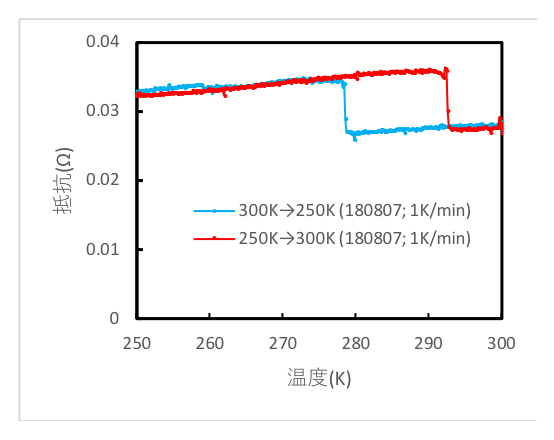
\includegraphics[width=100mm]{resistance250-300.eps}
  \end{center}
  \caption{抵抗の温度依存性}
  \label{fig:resistance250-300}
   \end{minipage}
 \begin{minipage}{0.3\hsize}
  \begin{center}
   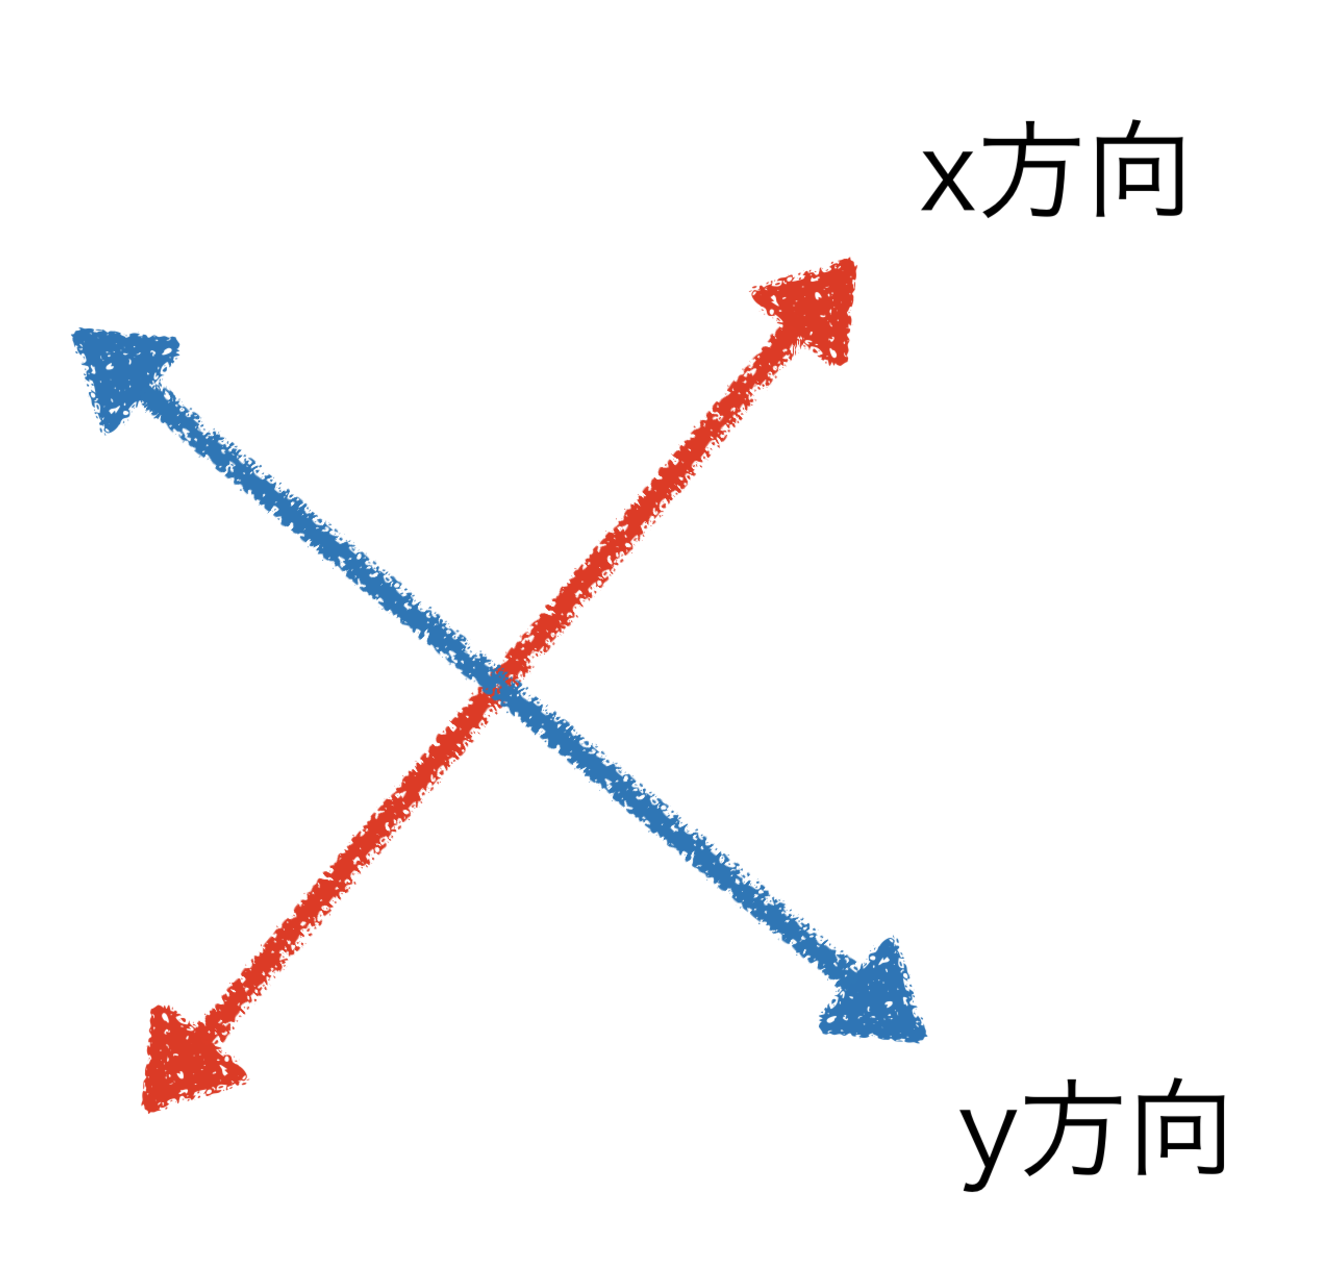
\includegraphics[width=50mm]{xy.eps}
  \end{center}
  \caption{偏光のx方向とy方向}
  \label{fig:xy}
  \end{minipage}
\end{figure}

\begin{figure}[htb]
 \begin{minipage}{0.333\hsize}
  \begin{center}
   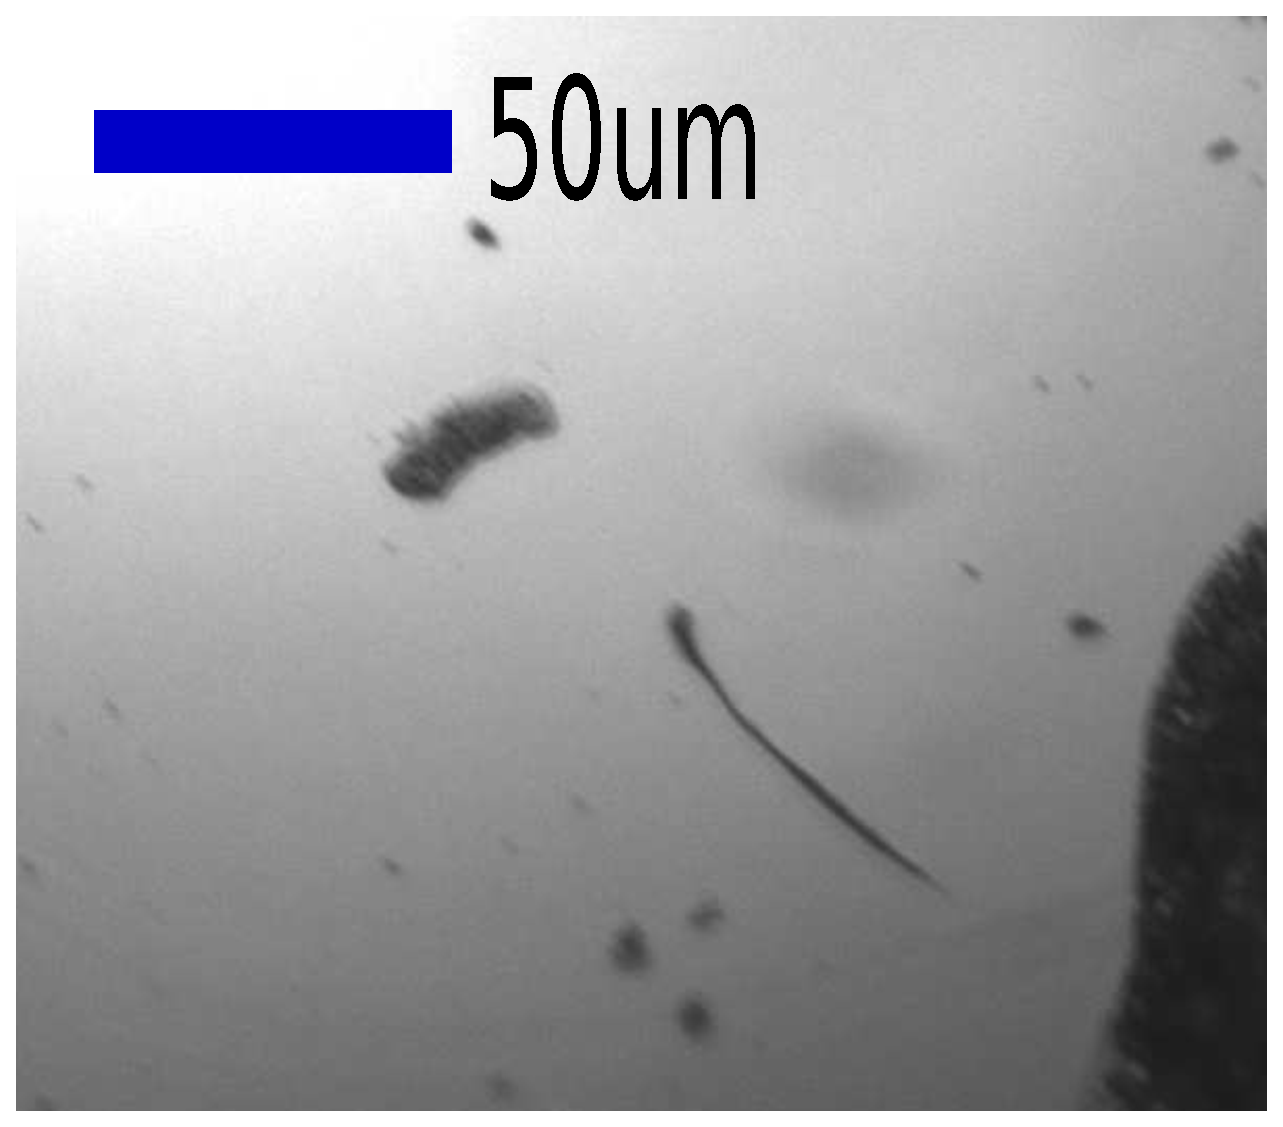
\includegraphics[width=\hsize]{nonpol300.eps}
  \end{center}
  \caption{無偏光@300K}
  \label{fig:nonpol300}
 \end{minipage}
 \begin{minipage}{0.333\hsize}
  \begin{center}
   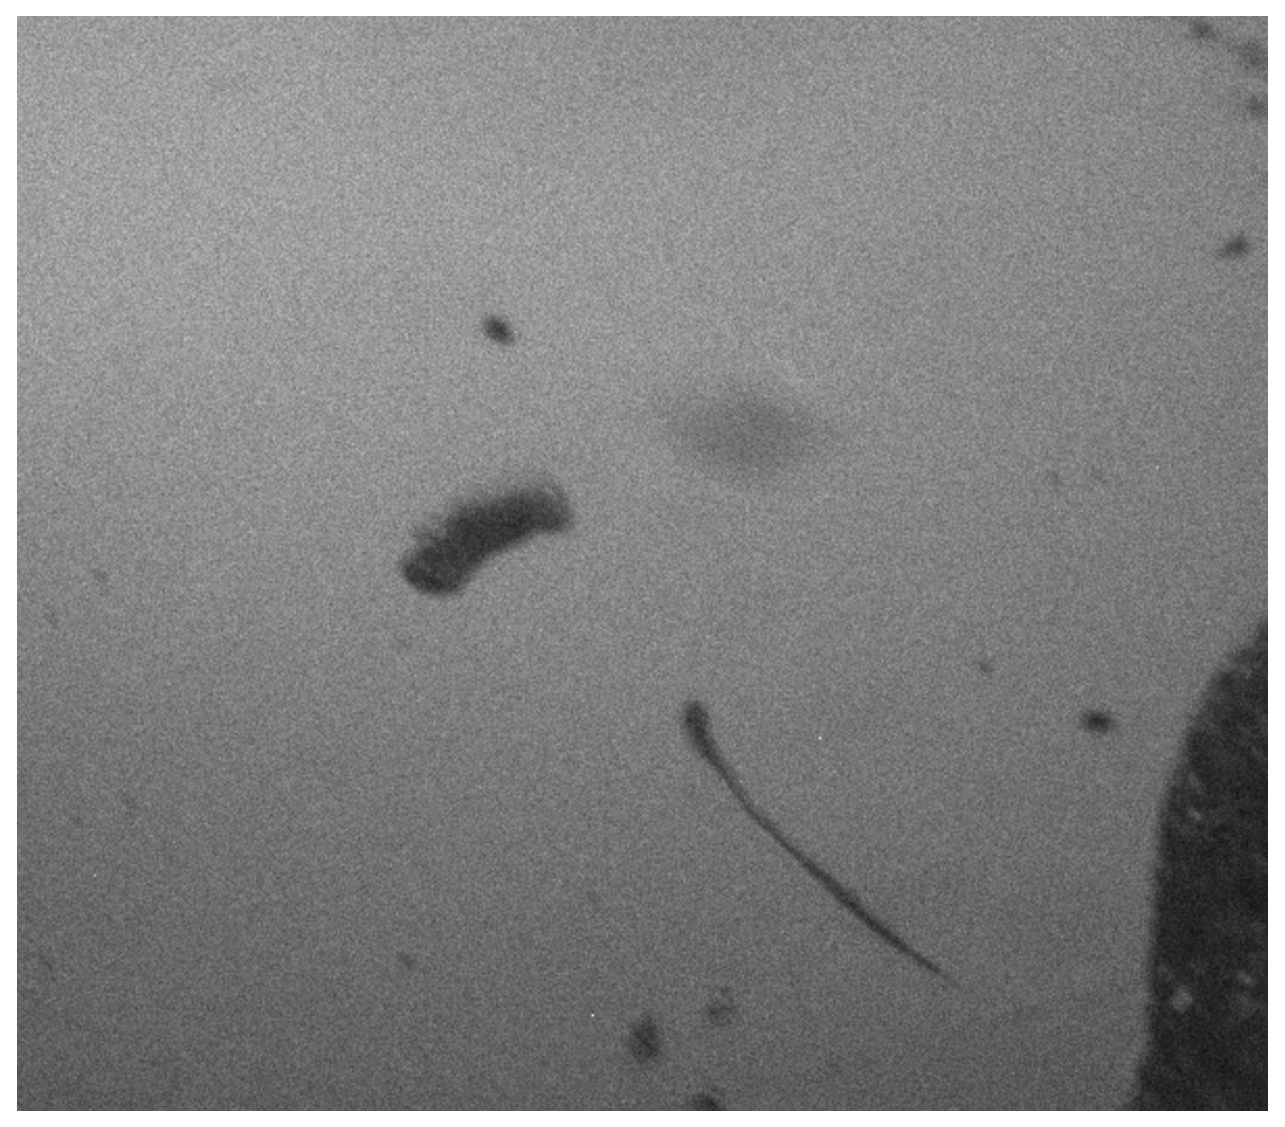
\includegraphics[width=\hsize]{hh300.eps}
  \end{center}
  \caption{平行偏光(x偏光/x検出)@300K}
  \label{fig:hh300}
 \end{minipage}
 \begin{minipage}{0.333\hsize}
  \begin{center}
   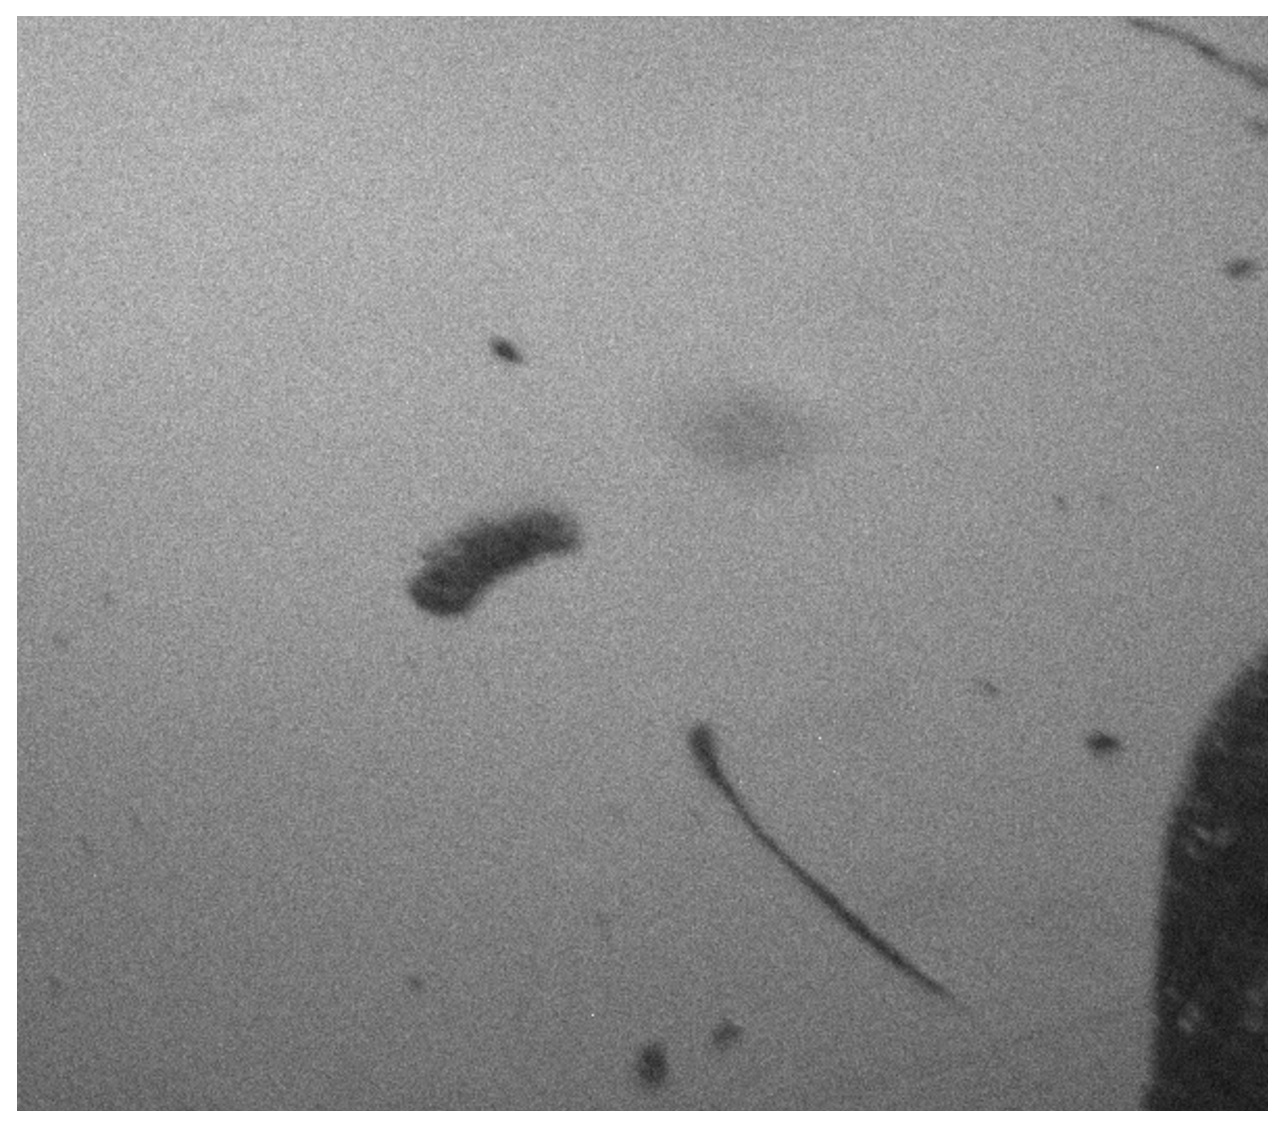
\includegraphics[width=\hsize]{vv300.eps}
  \end{center}
  \caption{平行偏光(y偏光/y検出)@300K}
  \label{fig:vv300}
 \end{minipage}
 \begin{minipage}{0.333\hsize}
  \begin{center}
   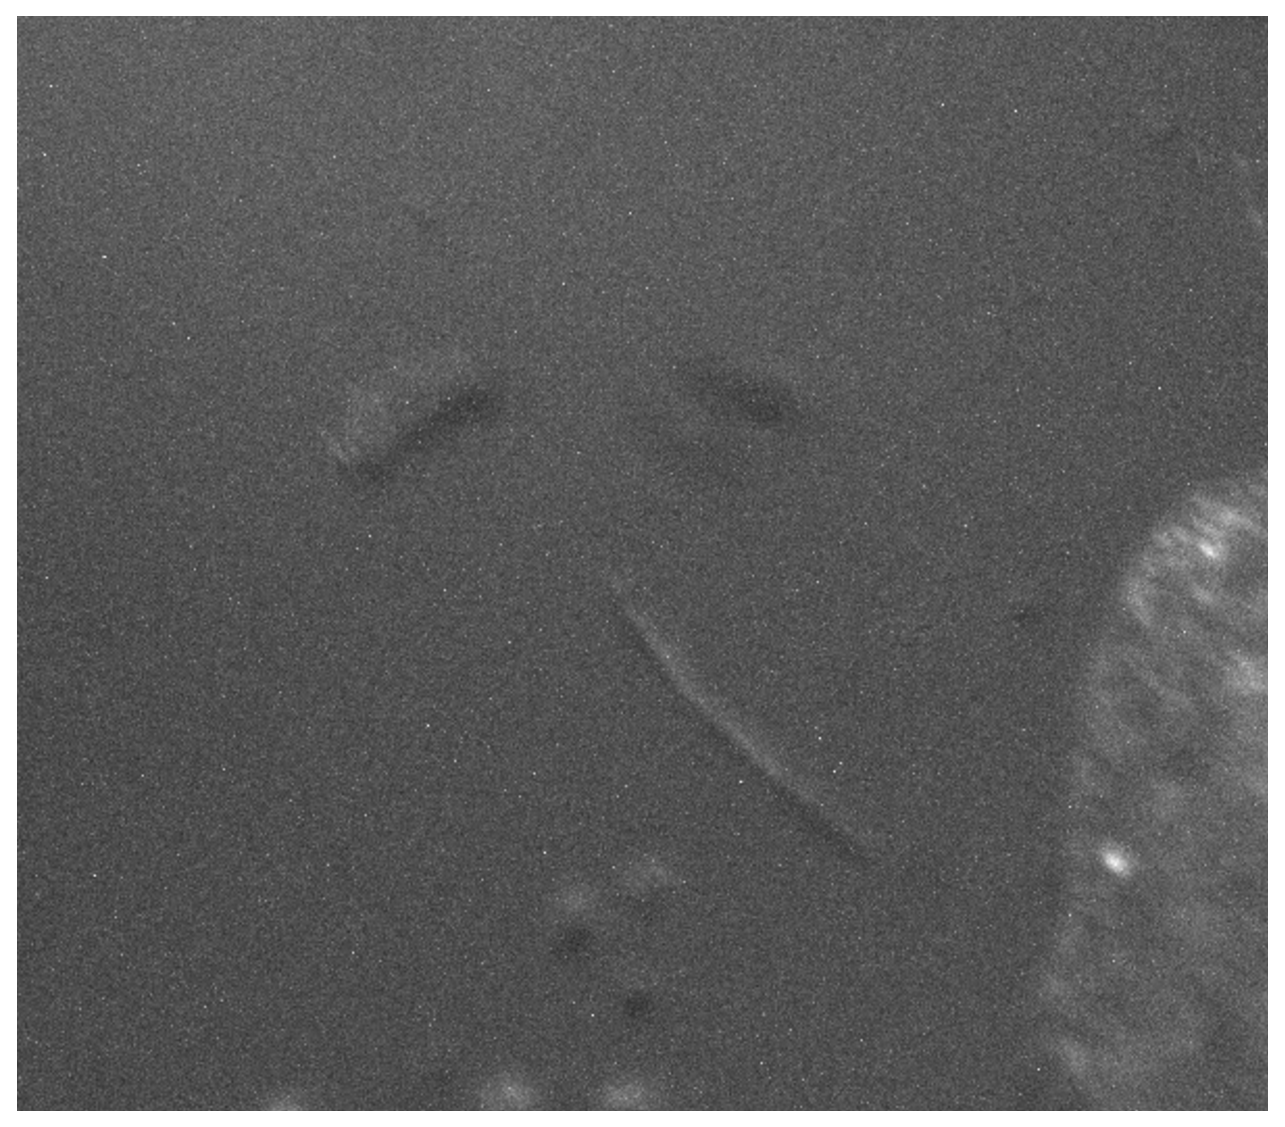
\includegraphics[width=\hsize]{vh300.eps}
  \end{center}
  \caption{直交偏光(y偏光/x検出)@300K}
  \label{fig:vh300}
 \end{minipage}
 \begin{minipage}{0.333\hsize}
  \begin{center}
   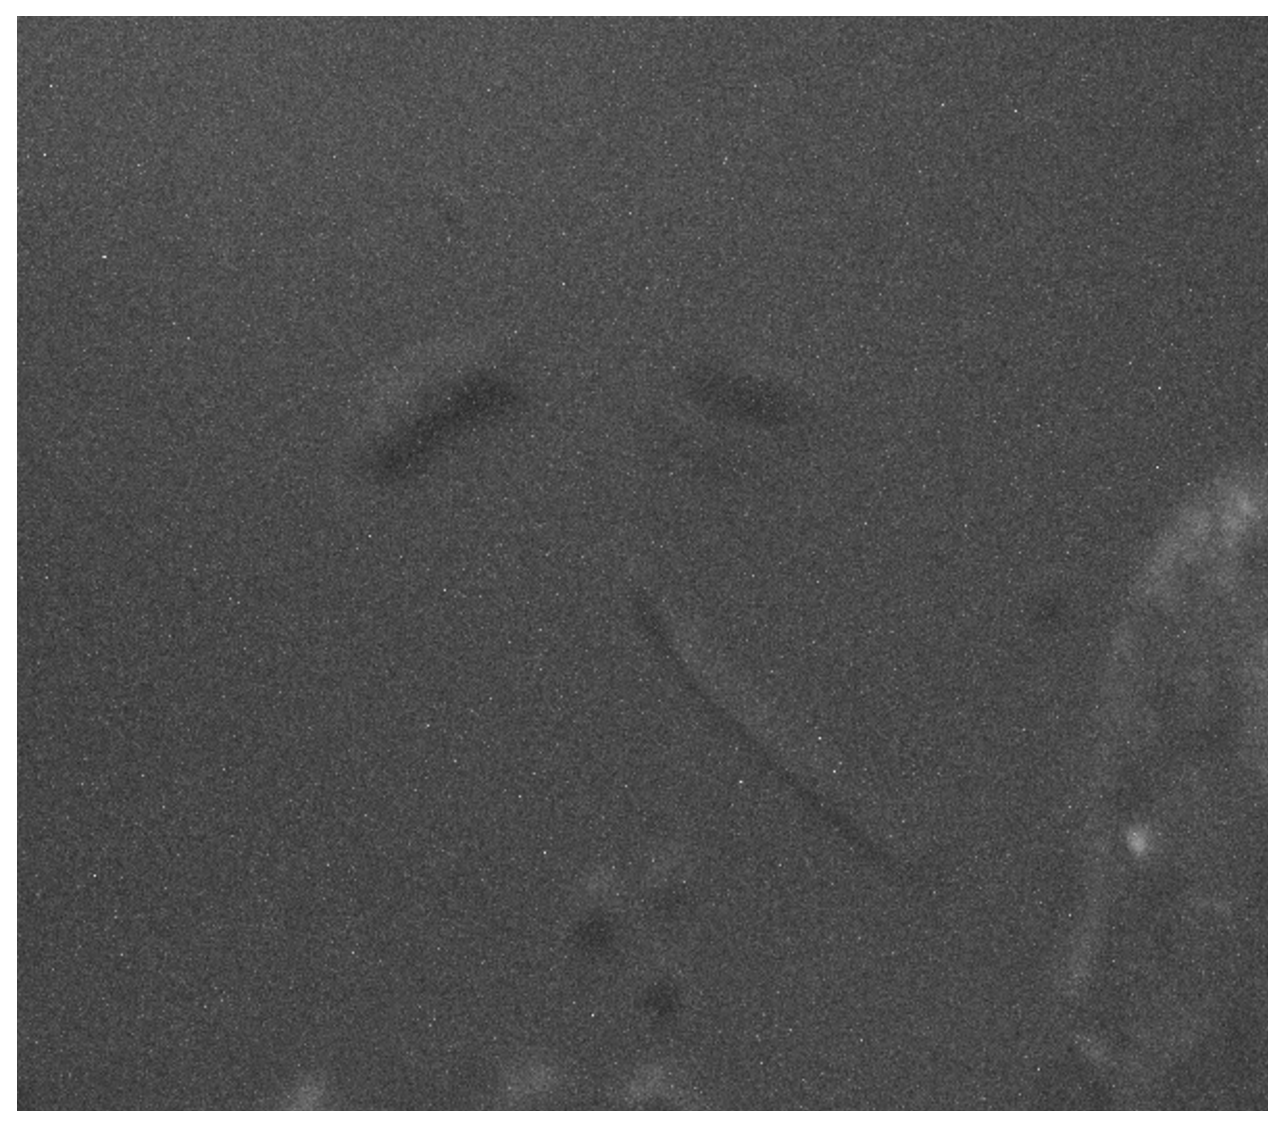
\includegraphics[width=\hsize]{hv300.eps}
  \end{center}
  \caption{直交偏光(x偏光/y検出)@300K}
  \label{fig:hv300}
 \end{minipage}
 \begin{minipage}{0.333\hsize}
  \begin{center}
   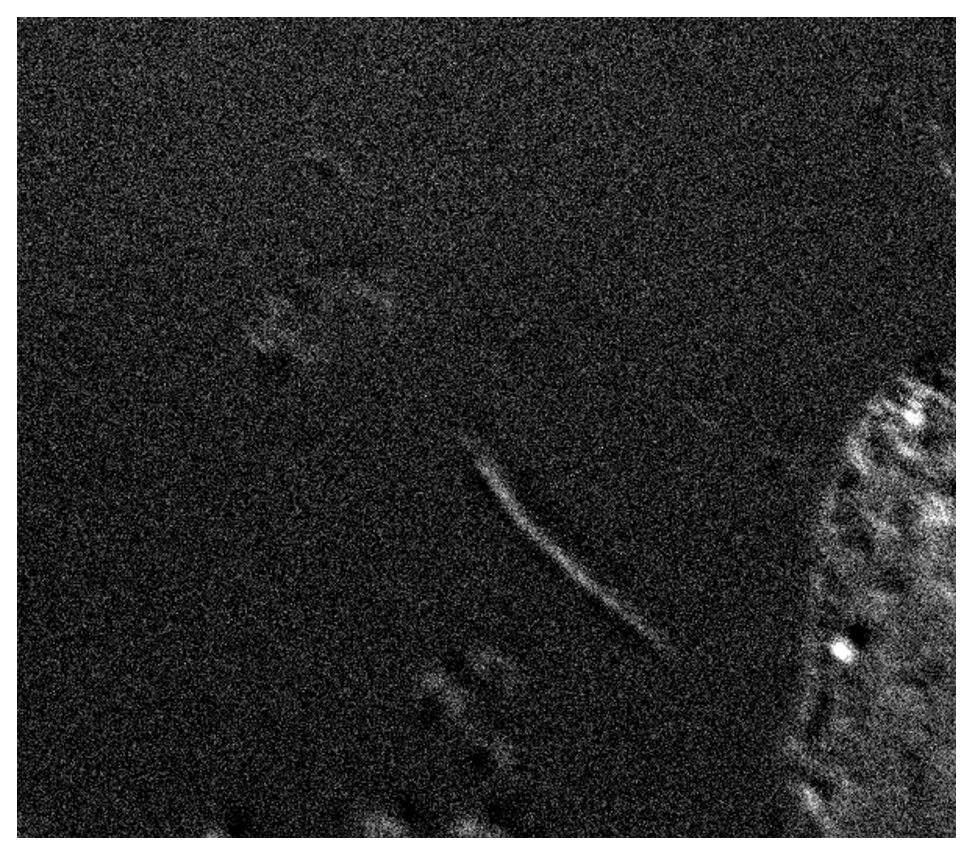
\includegraphics[width=\hsize]{vh300_subtractedby_hv300.eps}
  \end{center}
  \caption{図\ref{fig:vh300}と図\ref{fig:hv300}の差分@300K}
  \label{fig:vh300_subtractedby_hv300}
 \end{minipage}
 \begin{minipage}{0.333\hsize}
  \begin{center}
   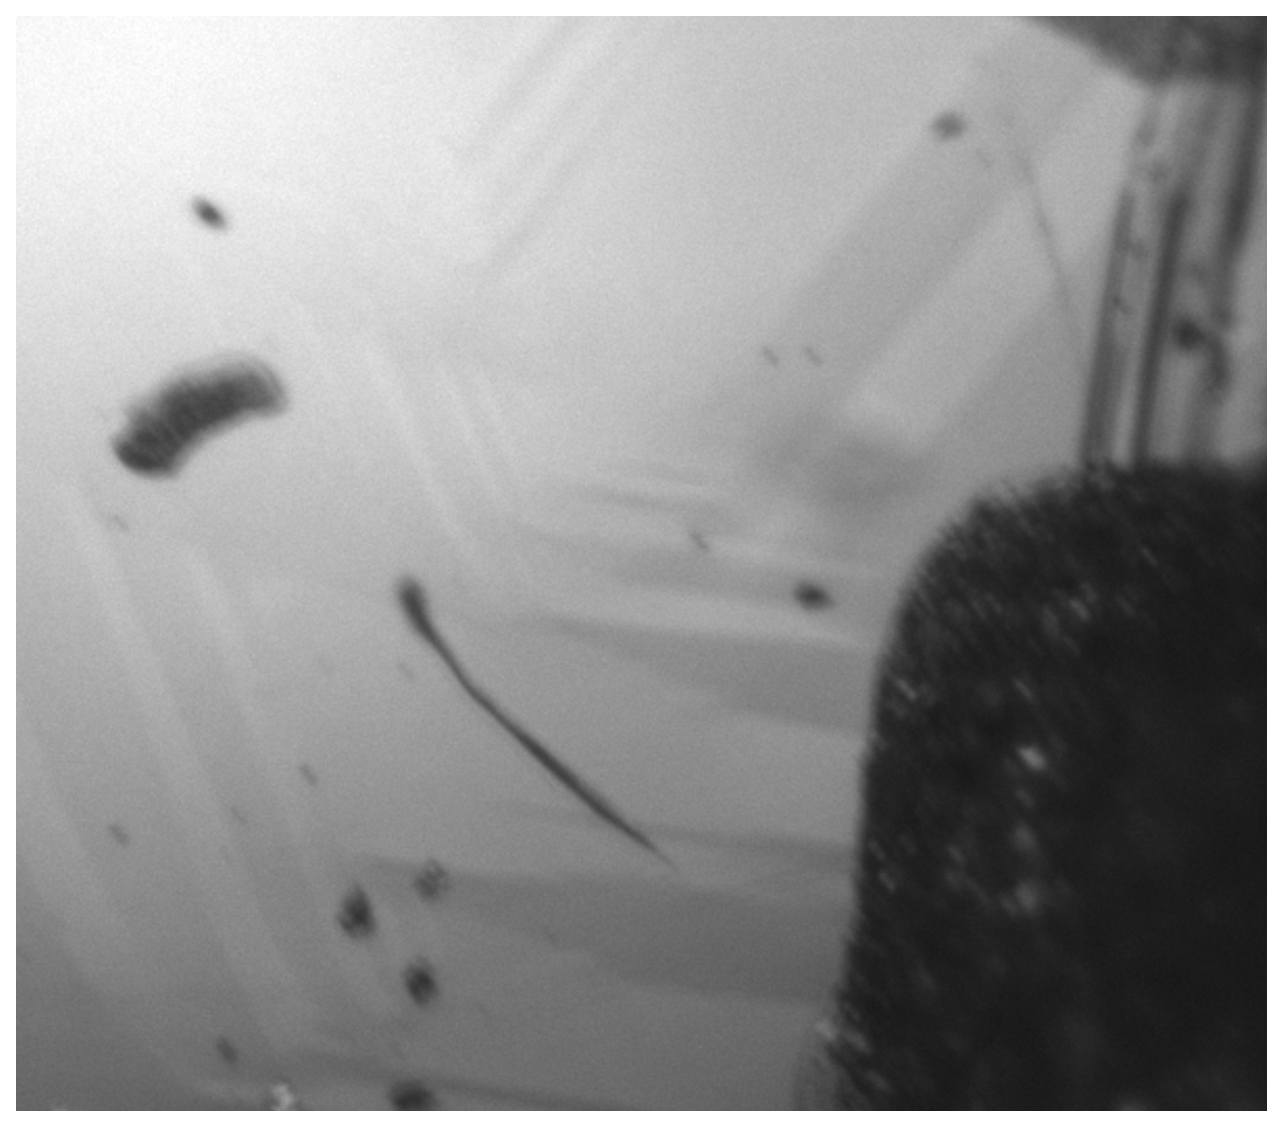
\includegraphics[width=\hsize]{nonpol250.eps}
  \end{center}
  \caption{無偏光@250K}
  \label{fig:nonpol250}
 \end{minipage}
 \begin{minipage}{0.333\hsize}
  \begin{center}
   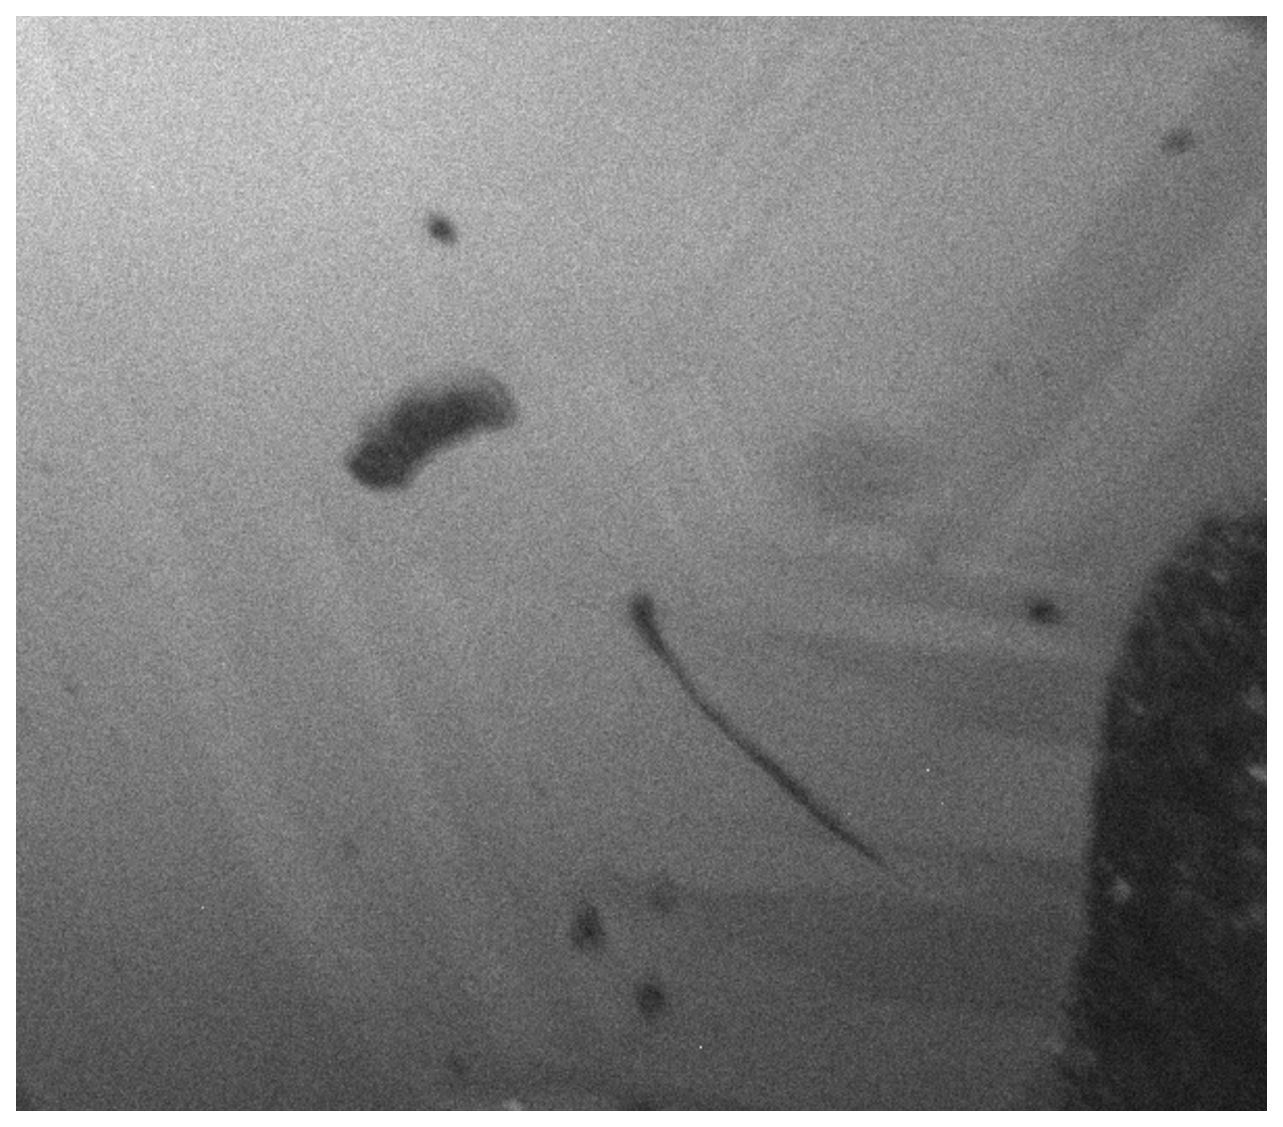
\includegraphics[width=\hsize]{hh250.eps}
  \end{center}
  \caption{平行偏光(x偏光/x検出)@250K}
  \label{fig:hh250}
 \end{minipage}
 \begin{minipage}{0.333\hsize}
  \begin{center}
   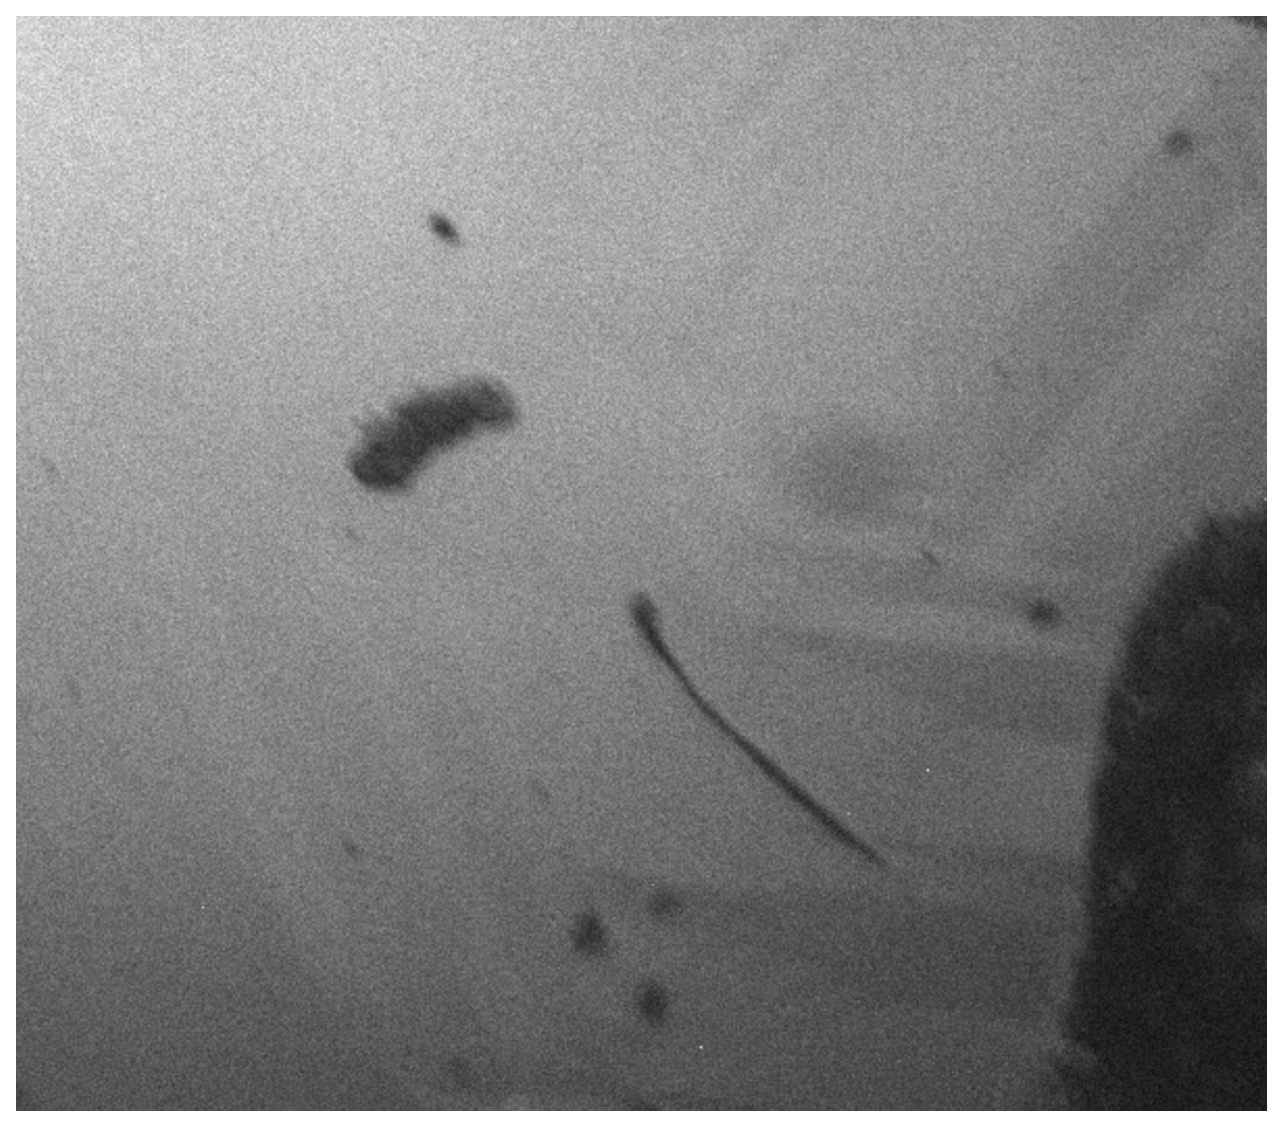
\includegraphics[width=\hsize]{vv250.eps}
  \end{center}
  \caption{平行偏光(y偏光/y検出)@250K}
  \label{fig:vv250}
 \end{minipage}
 \begin{minipage}{0.333\hsize}
  \begin{center}
   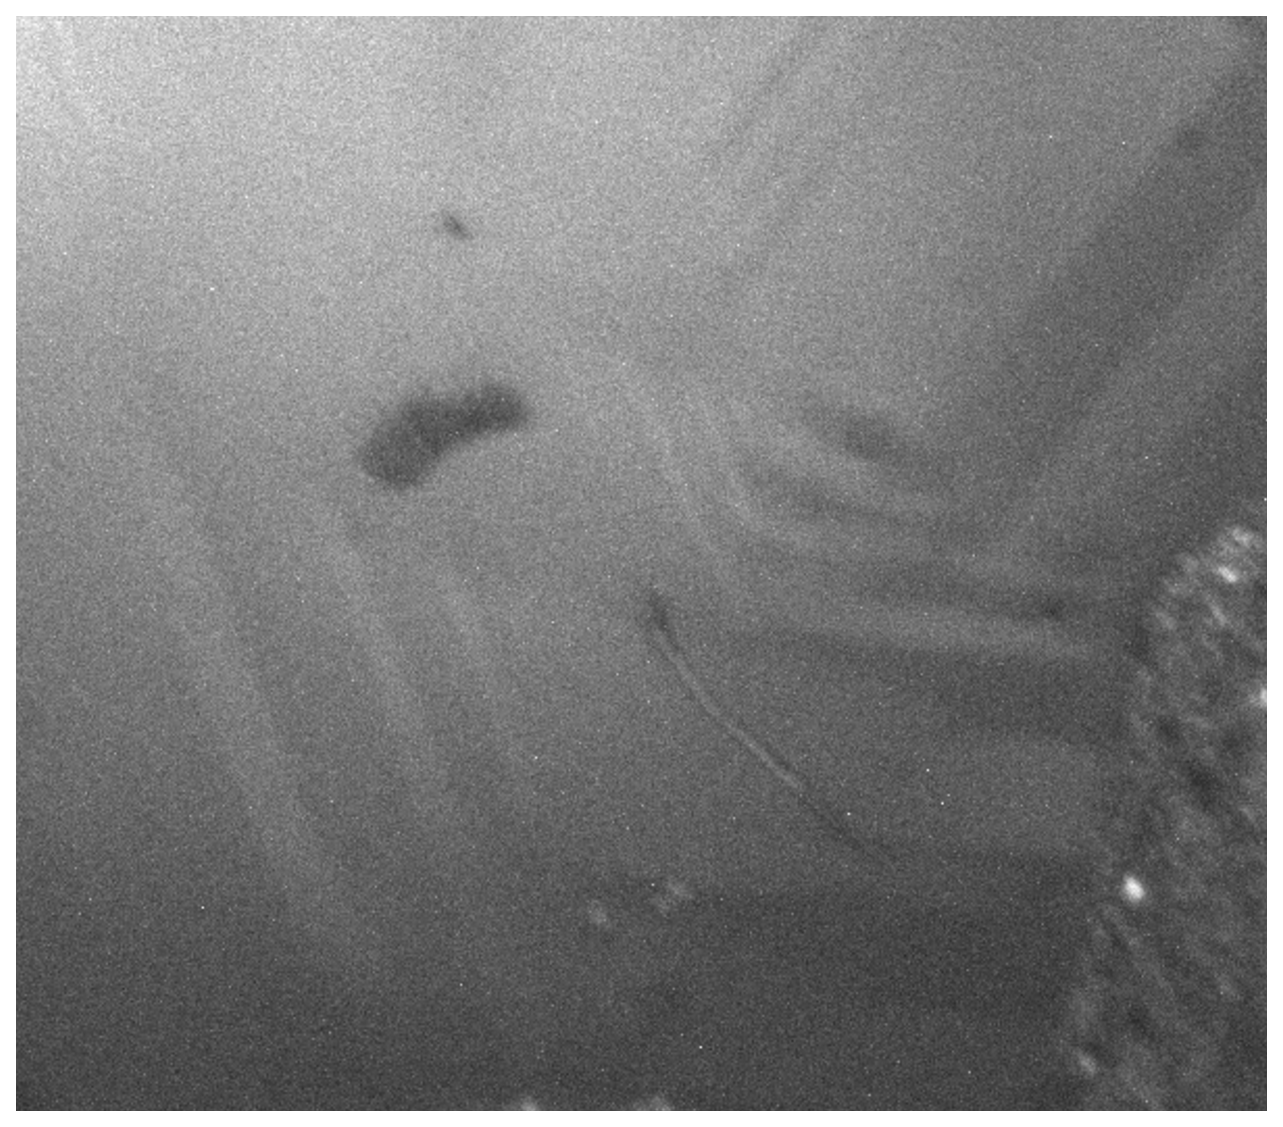
\includegraphics[width=\hsize]{vh250.eps}
  \end{center}
  \caption{直交偏光(y偏光/x検出)@250K}
  \label{fig:vh250}
 \end{minipage}
 \begin{minipage}{0.333\hsize}
  \begin{center}
   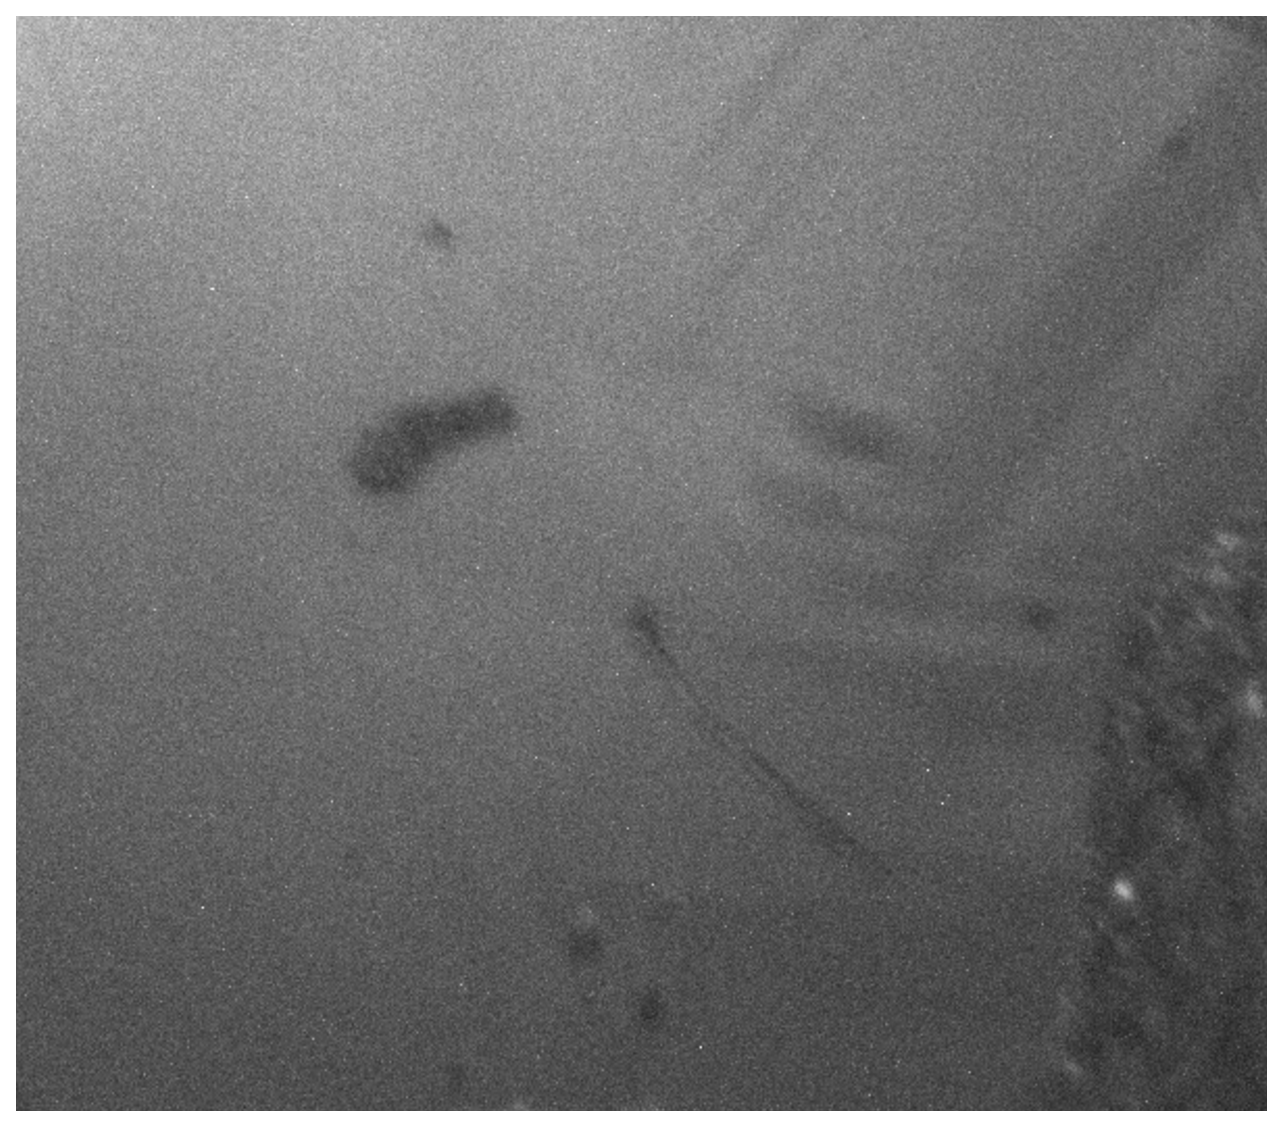
\includegraphics[width=\hsize]{hv250.eps}
  \end{center}
  \caption{直交偏光(x偏光/y検出)@250K}
  \label{fig:hv250}
 \end{minipage}
 \begin{minipage}{0.333\hsize}
  \begin{center}
   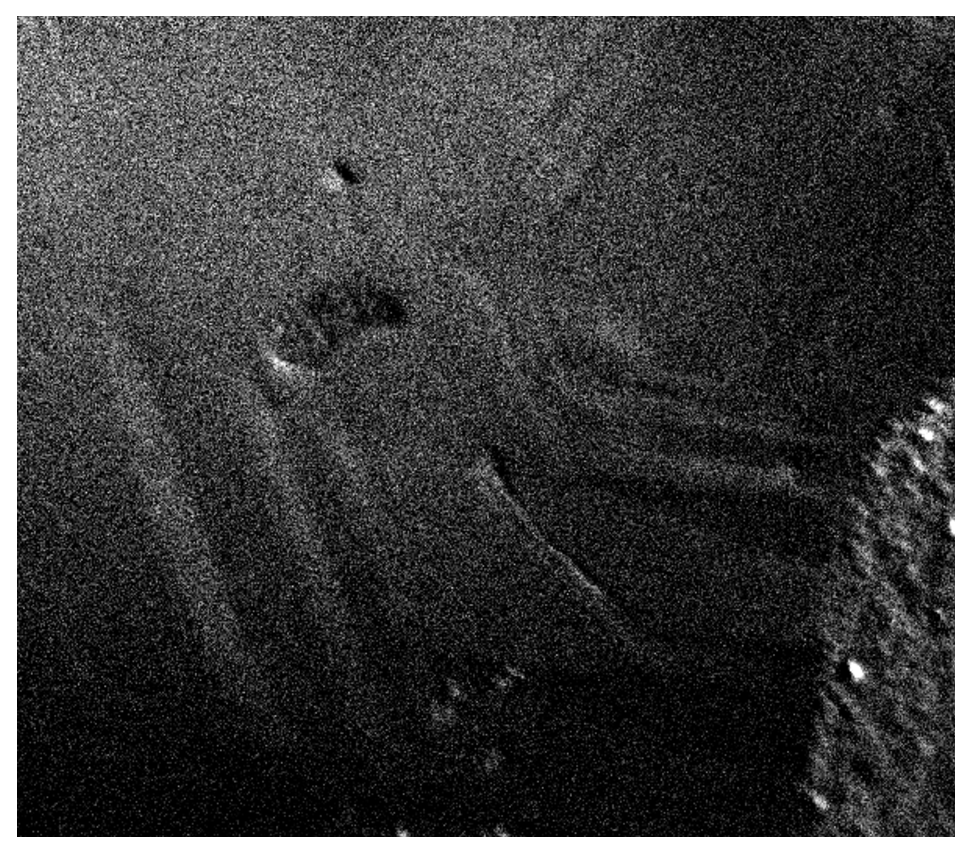
\includegraphics[width=\hsize]{vh250_subtractedby_hv250.eps}
  \end{center}
  \caption{図\ref{fig:vh250}と図\ref{fig:hv250}の差分@250K}
  \label{fig:vh250_subtractedby_hv250}
 \end{minipage}
\end{figure}

\begin{figure}[htb]
  \begin{center}
   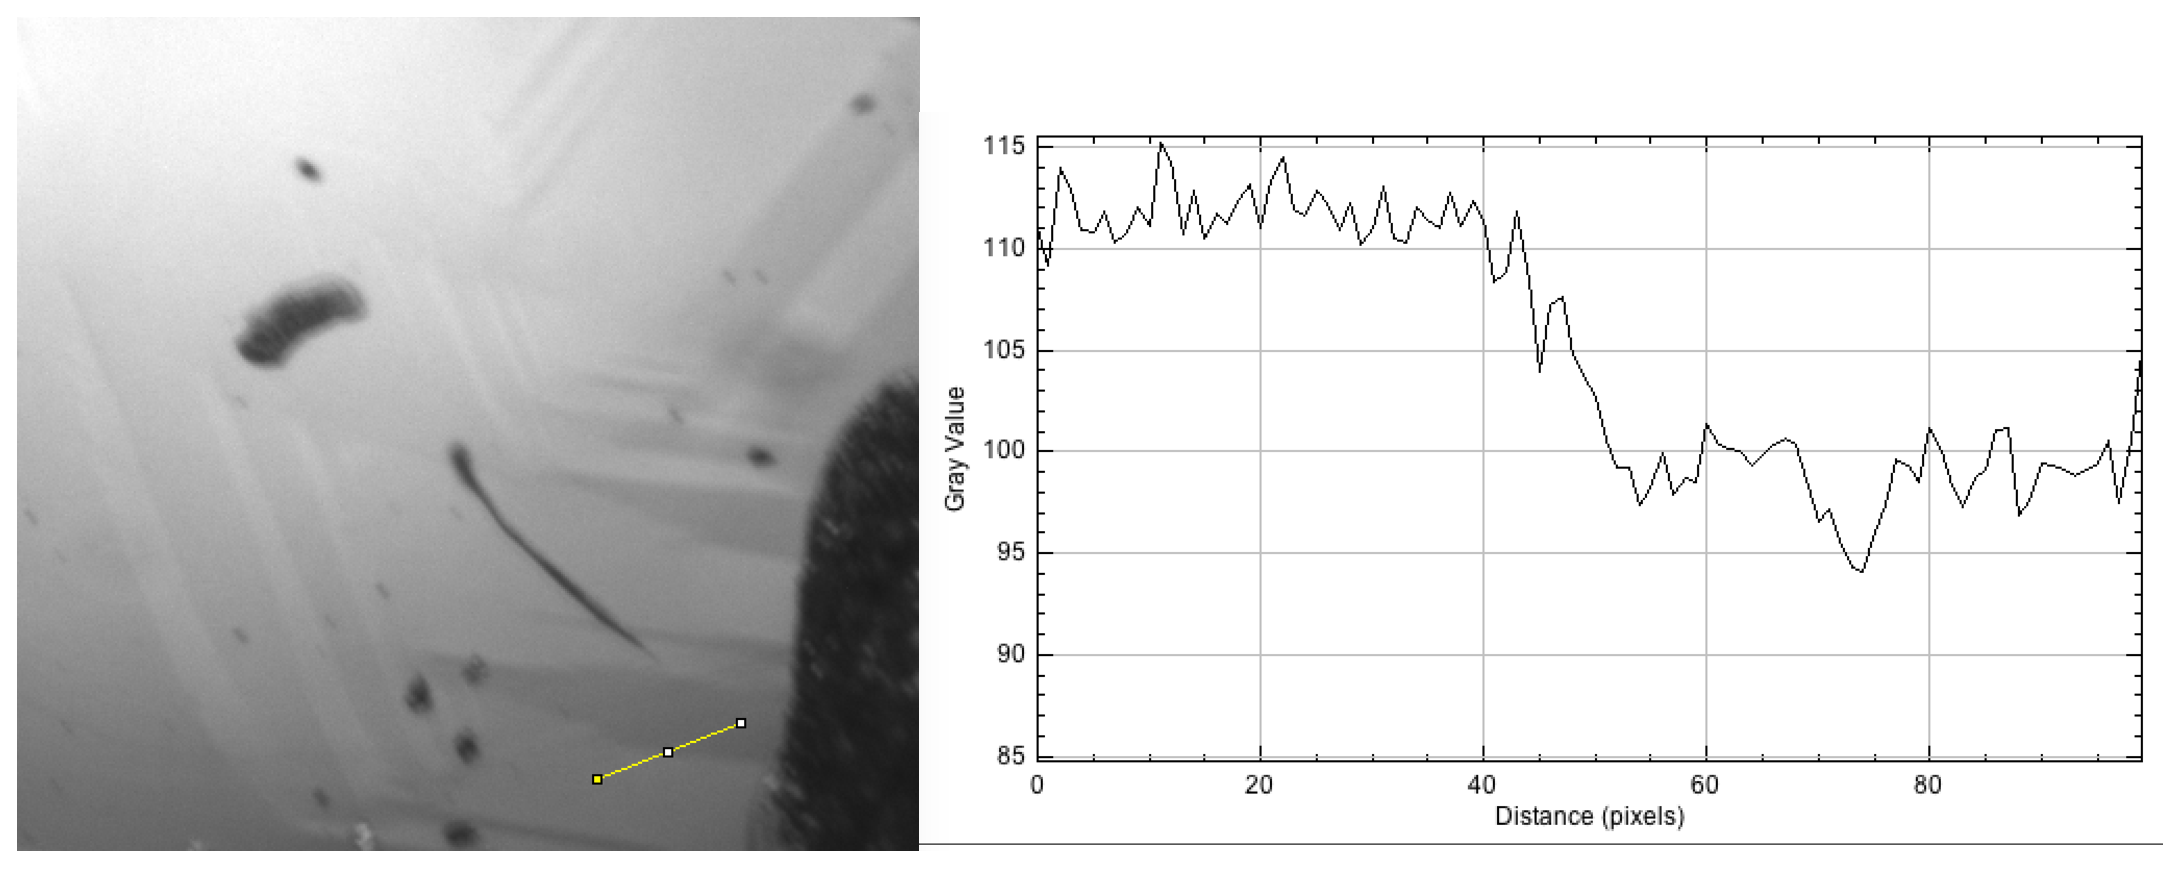
\includegraphics[width=0.8\hsize]{nonpol250_profile.eps}
  \end{center}
  \caption{信号強度のプロファイル(無偏光)@250K}
  \label{fig:nonpol250_profile}
\end{figure}

\subsection{250Kと50Kの偏光顕微鏡像の比較}
低温相の比較をするために、試料の温度を室温300Kから50Kまでレート1K/minで冷却したあと、同一のレートで50Kから300Kまで加熱した。冷却・加熱レート1K/minは前節で250Kから300Kまで温度掃引したときと同一である。図\ref{fig:resistance50-300}に温度と抵抗のヒステリシス曲線を示す。冷却中は270K付近と110K付近で少なくとも2回、不連続に抵抗が変化した。加熱中は240K付近のなだらかで特徴的な抵抗変化と、280K付近の不連続な抵抗変化が見られる。

図\ref{fig:microscope}の偏光顕微光学系から偏光子を取り去り、検光子をy方向に調整した光学系で、試料の冷却中に250Kと100K、50Kで偏光顕微鏡写真をとった。図\ref{fig:nonpolv250}と図\ref{fig:nonpolv100}、図\ref{fig:nonpolv50}にそれぞれ示す。さらに図\ref{fig:microscope}の偏光顕微光学系から偏光子と検光子をともに取り去った光学系で、試料の加熱中に50Kと150K、250K、300Kで無偏光の顕微鏡写真をとった。図\ref{fig:nonpol50_2}と図\ref{fig:nonpol150_2}、図\ref{fig:nonpol250_2}、図\ref{fig:nonpol300_2}にそれぞれ示す。一連の顕微鏡像は、前節の顕微鏡像と同一の領域を同じ倍率で撮影したものである。光源の明るさとCCDの動作条件は、図\ref{fig:nonpolv250}と図\ref{fig:nonpolv100}と図\ref{fig:nonpolv50}で同一であり、また図\ref{fig:nonpol50_2}と図\ref{fig:nonpol150_2}と図\ref{fig:nonpol250_2}と図\ref{fig:nonpol300_2}で同一である。ただし前節の顕微鏡像に比べて、光源の明るさとCCDの動作条件、光学系のセットアップが異なる。

検光子のみの条件で撮影した図\ref{fig:nonpolv250}は前節の250Kで撮影した無偏光の条件(図\ref{fig:nonpol250})と平行偏光の条件(図\ref{fig:vv250})と光学実験の条件が異なるが、冷却のレート1K/minは同一である。これらの図を比較してみると、明らかに異なる明暗のパターンが現れていることが分かる。したがって300Kから250Kまで同一のレート1K/minで繰り返し冷却しても、顕微鏡写真に現れる明暗のパターンは再現しないことが分かる。

250Kで撮影した図\ref{fig:nonpolv250}と100Kで撮影した図\ref{fig:nonpolv100}を比較すると、冷却により明暗のパターンが変化し、コントラストが小さくなったことが分かる。

冷却中に図\ref{fig:nonpolv100}(100K)で観察された顕微鏡写真に特徴的なパターンは、検光子のみの光学系で撮影された図\ref{fig:nonpolv50}(50K)と無偏光の光学系で撮影された図\ref{fig:nonpol50_2}(50K)でともに観察される。新しく現れた低温相に特徴的なパターンは、図\ref{fig:nonpol250_2}から分かるように加熱していったとき遅くとも250Kまで保たれた。

最後に本節で得られた結果をまとめる。
\begin{enumerate}
\item 300Kから250Kまで同一のレート1K/minで繰り返し冷却しても、顕微鏡写真に現れる明暗のパターンは再現しない
\item 250Kから100Kまでレート1K/minで冷却してゆき、冷却前後で顕微鏡写真を比較すると、明暗のパターンが変化し、コントラストが小さくなった(図\ref{fig:nonpolv250}、図\ref{fig:nonpolv100})
\item 50Kの低温相の顕微鏡写真に特徴的な明暗のパターンは、加熱してゆくと250Kでも保たれた(図\ref{fig:nonpol50_2}、図\ref{fig:nonpol150_2}、図\ref{fig:nonpol250_2})
 \end{enumerate}

\begin{figure}[htb]
  \begin{center}
   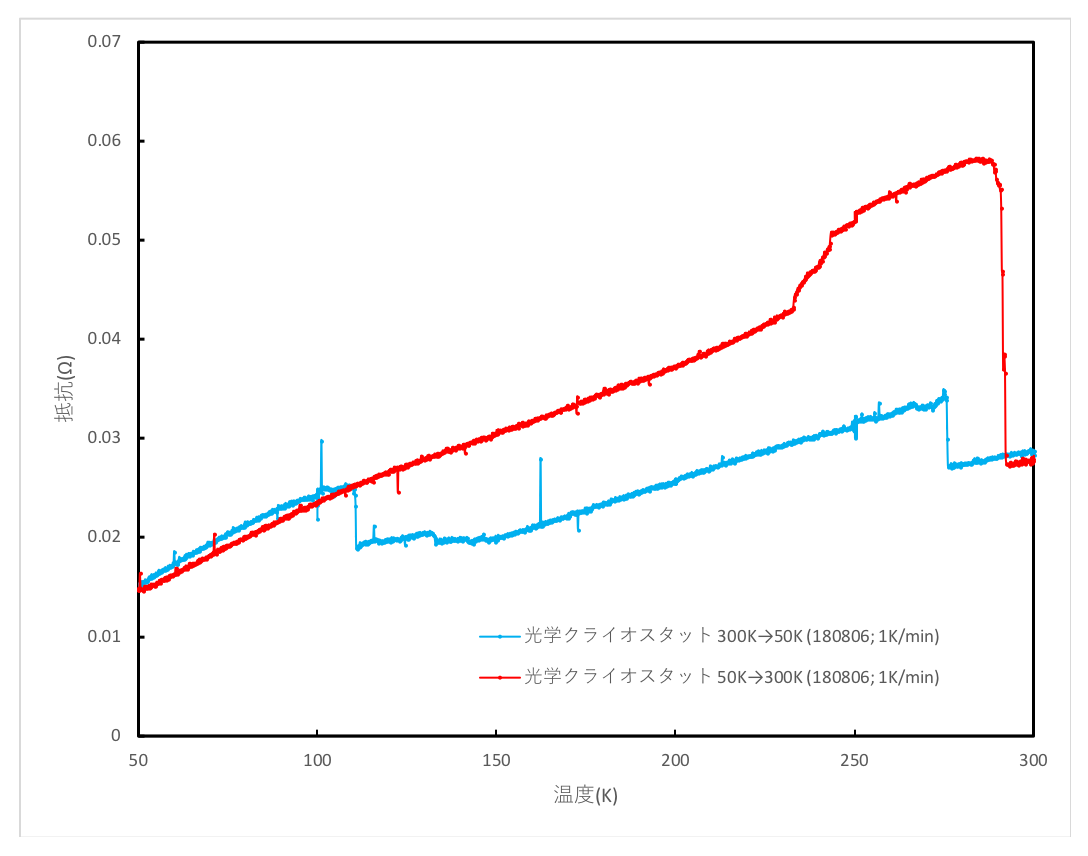
\includegraphics[width=150mm]{resistance50-300.eps}
  \end{center}
  \caption{抵抗の温度依存性}
  \label{fig:resistance50-300}
\end{figure}

\begin{figure}[htb]
 \begin{minipage}{0.333\hsize}
  \begin{center}
   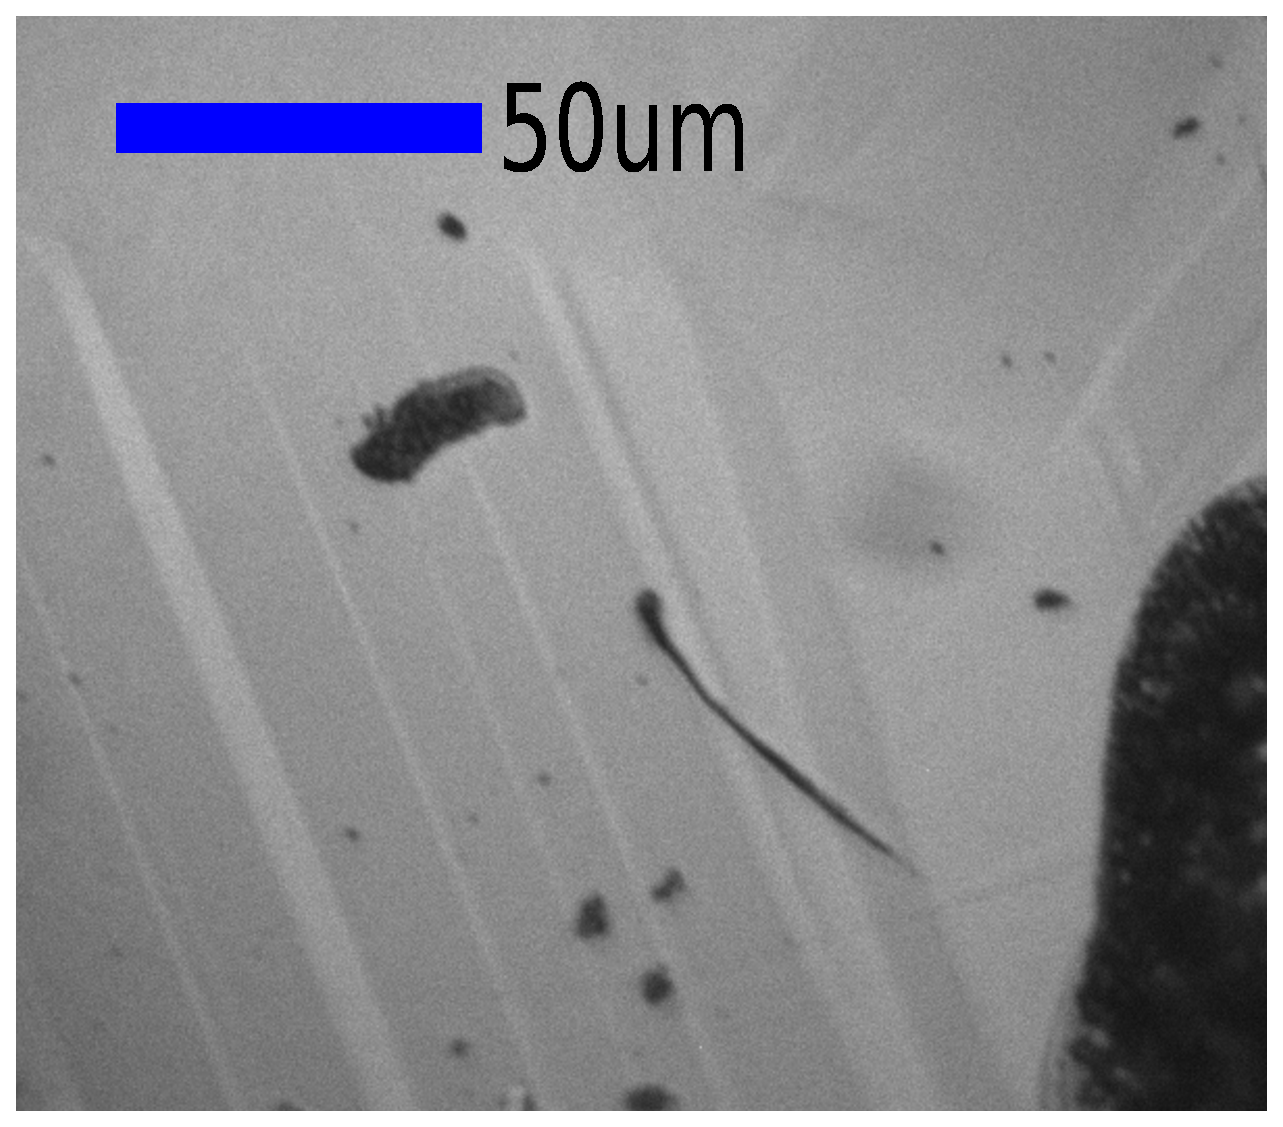
\includegraphics[width=\hsize]{nonpolv250.eps}
  \end{center}
  \caption{検光子のみ(y検出)@250K}
  \label{fig:nonpolv250}
 \end{minipage}
 \begin{minipage}{0.333\hsize}
  \begin{center}
   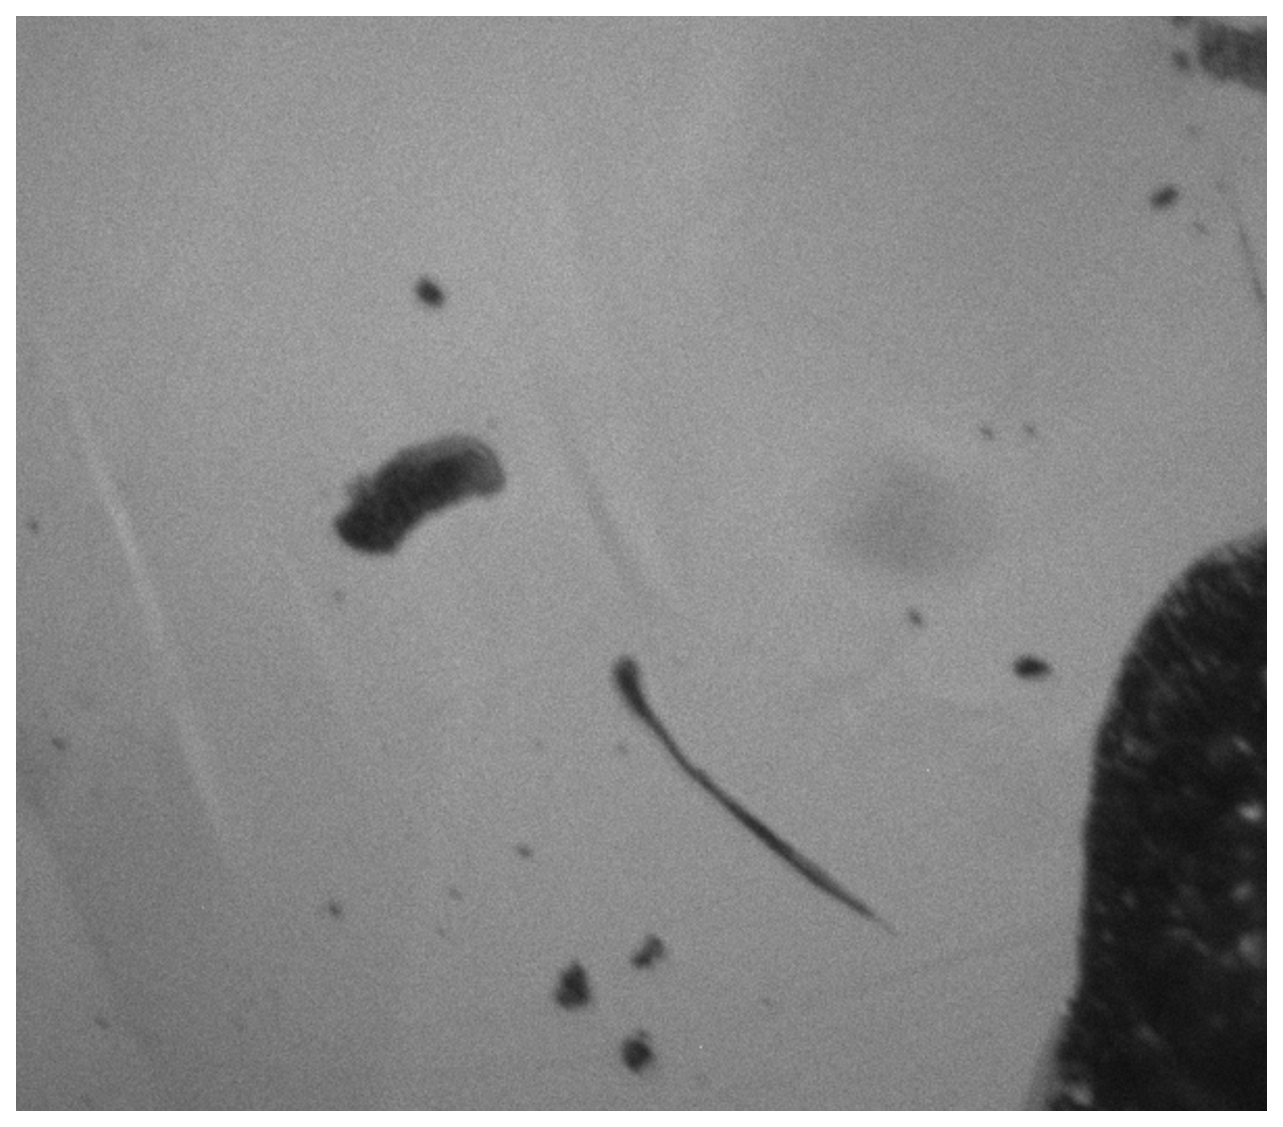
\includegraphics[width=\hsize]{nonpolv100.eps}
  \end{center}
  \caption{検光子のみ(y検出)@100K}
  \label{fig:nonpolv100}
 \end{minipage}
 \begin{minipage}{0.333\hsize}
  \begin{center}
   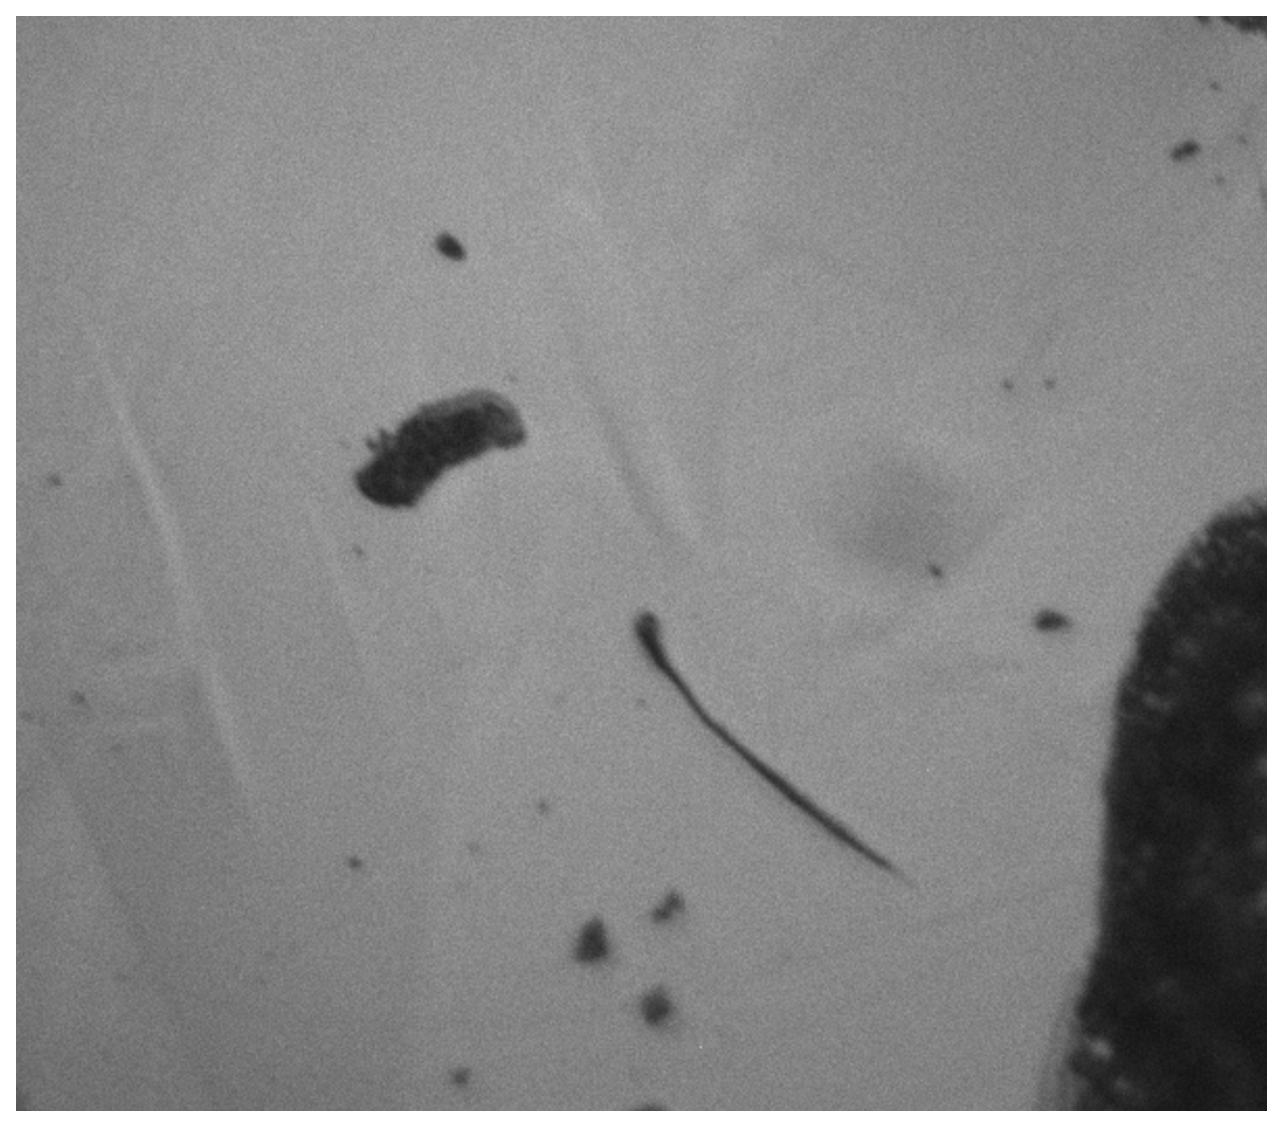
\includegraphics[width=\hsize]{nonpolv50.eps}
  \end{center}
  \caption{検光子のみ(y検出)@50K}
  \label{fig:nonpolv50}
 \end{minipage}
 \begin{minipage}{0.333\hsize}
  \begin{center}
   \includegraphics[width=\hsize]{nonpol50_2.eps}
  \end{center}
  \caption{無偏光@50K}
  \label{fig:nonpol50_2}
 \end{minipage}
  \begin{minipage}{0.333\hsize}
  \begin{center}
   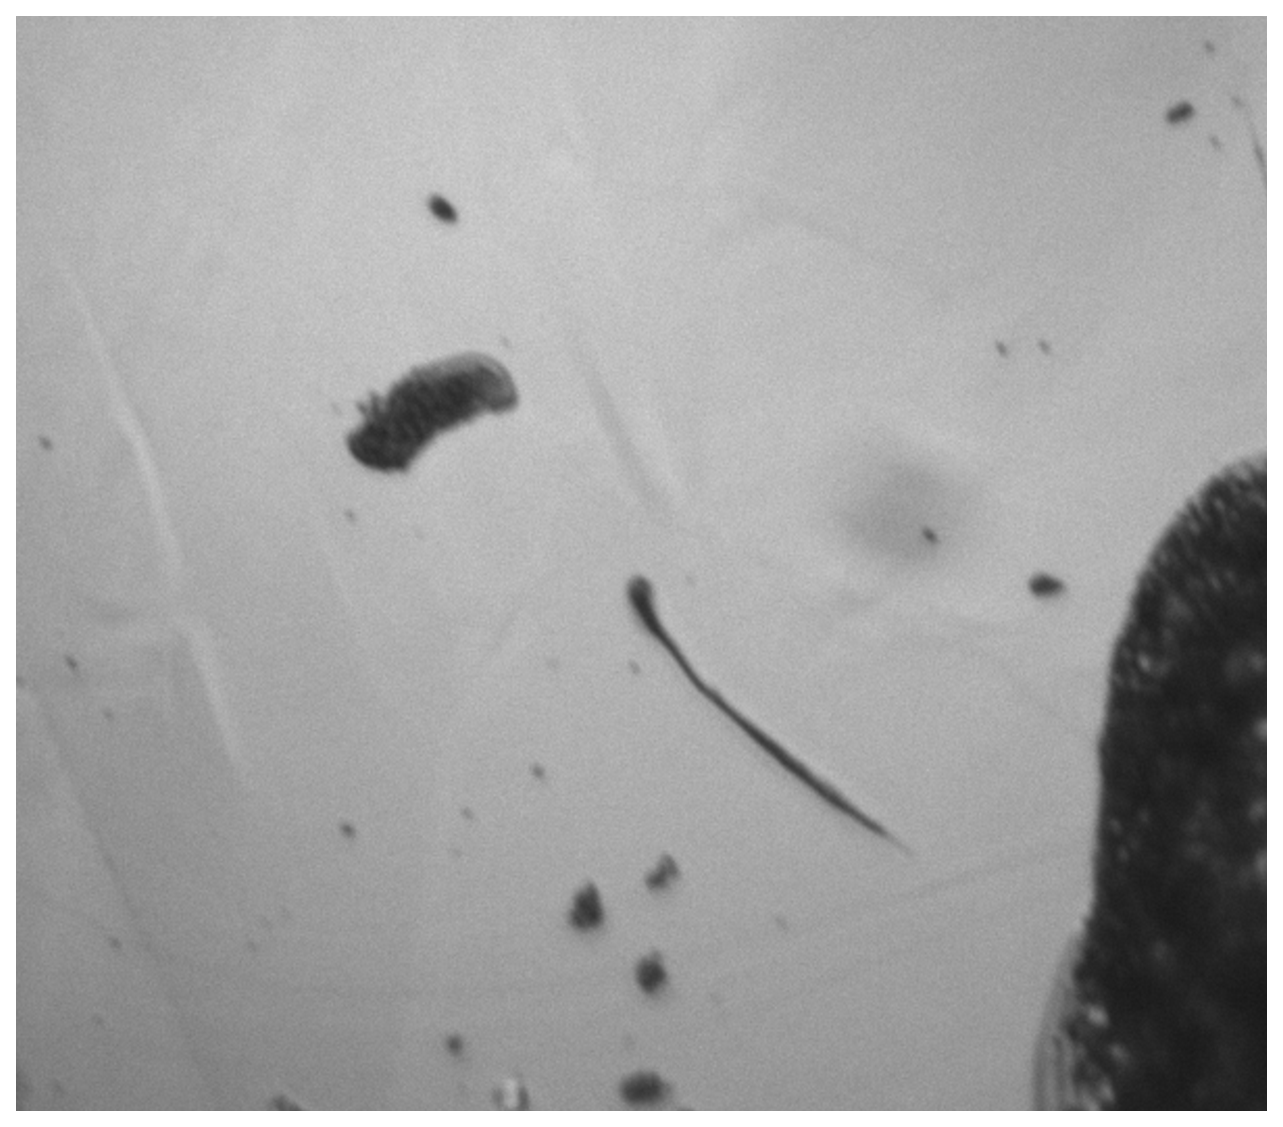
\includegraphics[width=\hsize]{nonpol150_2.eps}
  \end{center}
  \caption{無偏光@150K}
  \label{fig:nonpol150_2}
 \end{minipage}
 \begin{minipage}{0.333\hsize}
  \begin{center}
   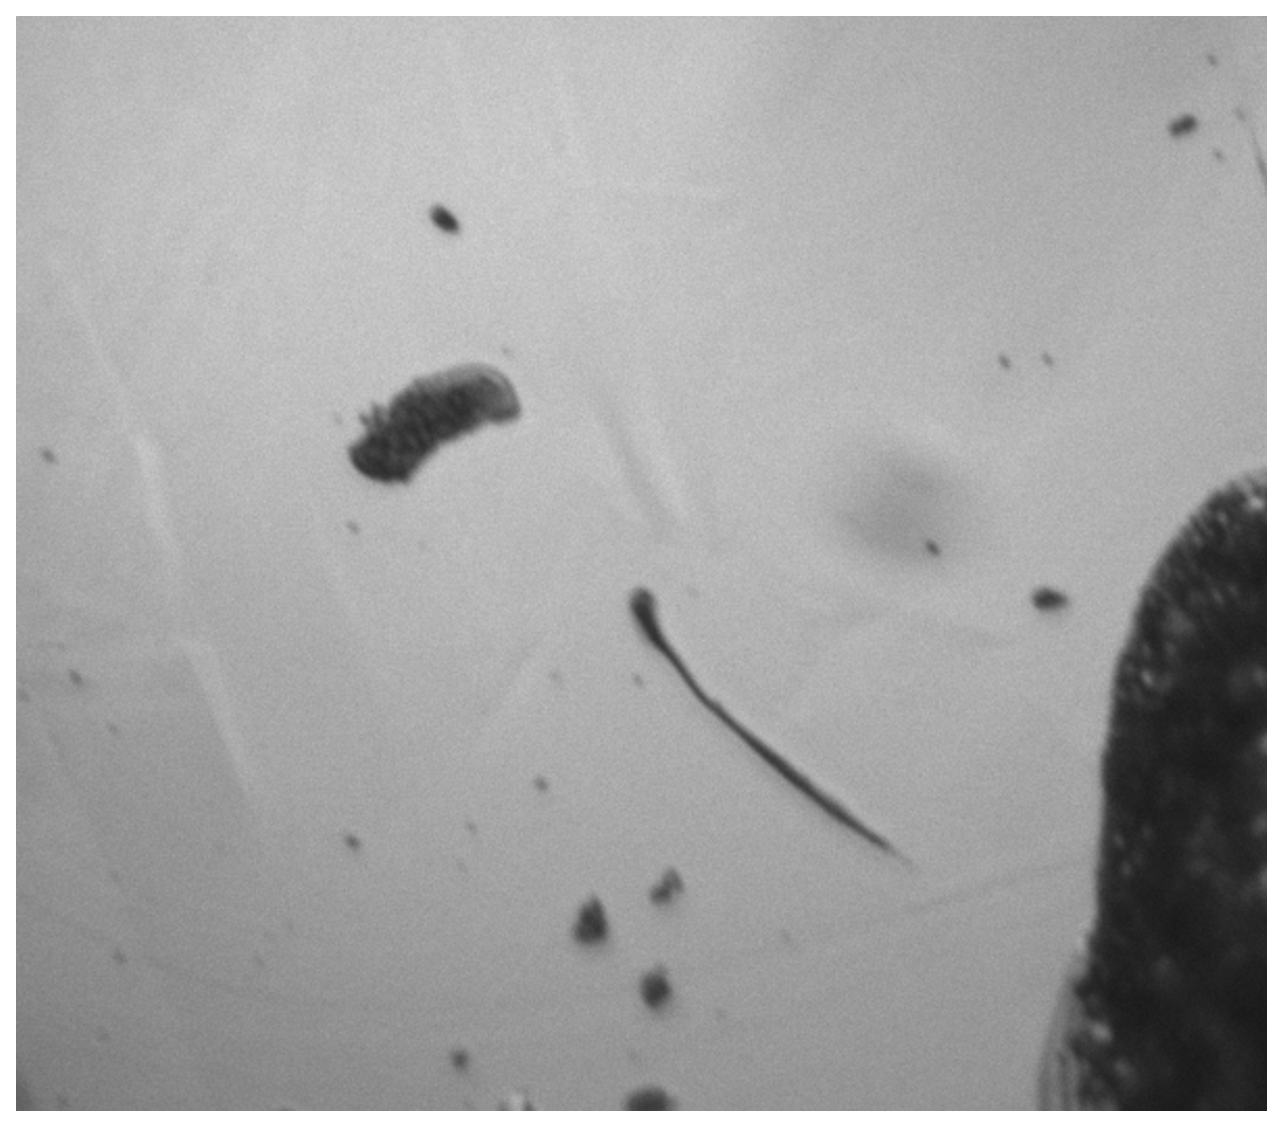
\includegraphics[width=\hsize]{nonpol250_2.eps}
  \end{center}
  \caption{無偏光@250K}
  \label{fig:nonpol250_2}
 \end{minipage}
 \begin{minipage}{0.333\hsize}
  \begin{center}
   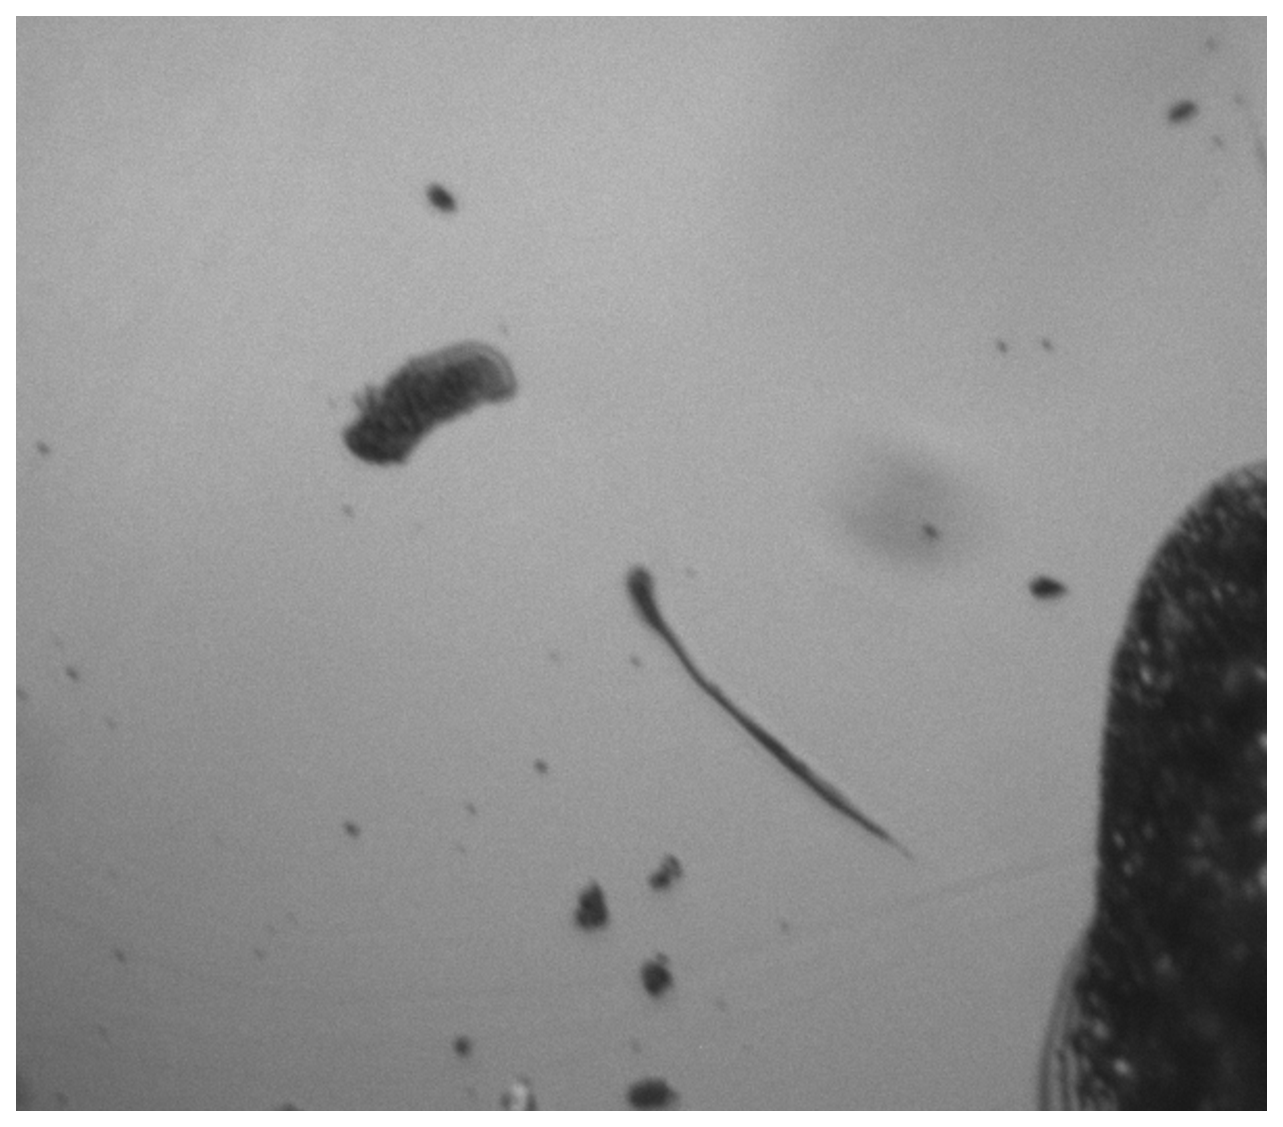
\includegraphics[width=\hsize]{nonpol300_2.eps}
  \end{center}
  \caption{無偏光@300K}
  \label{fig:nonpol300_2}
 \end{minipage}
\end{figure}

\subsection{結果の考察}
偏光顕微鏡の観察から以下の結果が得られた。
\begin{description}
\item[300Kと250Kの偏光顕微鏡像の比較]
\item
\begin{enumerate}
\item 300Kから250Kまでレート1K/minで冷却してゆくと、300Kの顕微鏡写真に見られなかった明暗のパターンが、250Kの顕微鏡写真に現れた。その明暗のパターンは無偏光の条件(図\ref{fig:nonpol250})と平行偏光偏光条件(図\ref{fig:hh250}、\ref{fig:vv250})、直交偏光条件(図\ref{fig:vh250}、\ref{fig:hv250})の全条件に関して見て取れる。ただしコントラストは条件により異なる。
\item 明るい領域は、典型的に細長い形をしており、概ね$10 \mu m$オーダーの大きさを持つ。また明るい領域と暗い領域の境界の方向は三方向あり、お互いに概ね60度の角度をなしている。
\item 明るい領域と暗い領域の境界で信号強度は急峻に変化した。無偏光の条件で明るい領域と暗い領域のコントラストは13\%程度である(図\ref{fig:nonpol250_profile})
\item 直交偏光の条件で250Kの明るい領域は、周囲と比べて明るいだけでなく300Kの対応する領域に対しても明るい(図\ref{fig:vh300}、\ref{fig:vh250})
\item 直交偏光の条件で、明るく細長い領域が伸びる方向と偏光/検光方向に依存して周囲との明暗のコントラストが異なる(図\ref{fig:vh250} 、\ref{fig:hv250})
 \end{enumerate}
\item[250Kと50Kの偏光顕微鏡像の比較]
\item 
\begin{enumerate}
\item 300Kから250Kまで同一のレート1K/minで繰り返し冷却しても、顕微鏡写真に現れる明暗のパターンは再現しない
\item 250Kから100Kまでレート1K/minで冷却してゆき、冷却前後で顕微鏡写真を比較すると、明暗のパターンが変化し、コントラストが小さくなった(図\ref{fig:nonpolv250}、図\ref{fig:nonpolv100})
\item 50Kの低温相の顕微鏡写真に特徴的な明暗のパターンは、加熱してゆくと250Kでも保たれた(図\ref{fig:nonpol50_2}、図\ref{fig:nonpol150_2}、図\ref{fig:nonpol250_2})
 \end{enumerate}
 \end{description}
 
%%考察
得られた結果に関して以下のように筆者は考察する。
\begin{description}
\item[280K付近で現れた低温相に関して]
\item[]
試料を300Kから冷却してゆくと280K付近で、抵抗が不連続に変化し、顕微鏡像に明暗のパターンが現れた。また明暗のパターンの境界で、信号強度が急峻に変化した。これらの結果は少なくとも一部の領域に低温相が現れた証拠だと筆者は考える。この低温相に関して以下のことが言える:

\begin{description}
\item[低温相の異方性]
直交偏光の条件で250Kの明るい領域と300Kの対応する領域を比較すると、250Kの方が信号強度が強かった。これは低温相の明るい領域の異方的な反射率テンソルに起因する。また、直交偏光条件で偏光方向を変えると明るい領域と暗い領域のコントラストが変化した(図\ref{fig:vh250}、図\ref{fig:hv250})。この振る舞いは明るい領域と暗い領域の反射率がともに等方的であると仮定した場合、説明できない。したがって現れた低温相のうち少なくとも一部の領域で反射率テンソルは、異方的であることが確認できる。この異方的な反射率テンソルは、付録\ref{sec:IrTe2_reflectance_LT}で述べたように、低温相の結晶の対称性を反映したものである。
ただし、構築した光学系が理想的であると仮定すると、図\ref{fig:vh250}と図\ref{fig:hv250}の結果を説明できないことに注意する。付録\ref{sec:diagonazed_reflectance}より直交偏光条件で信号強度は、偏光子の回転に対して90度の周期性をもつ。一方、図\ref{fig:vh250}と図\ref{fig:hv250}は偏光子を90度回転させた条件に対応しており、一部の領域での信号強度の違いを説明できない。図\ref{fig:vh250}と図\ref{fig:hv250}の比較から観察されたコントラストの差は、光学系の問題と関連していると筆者は考える。

さらに、明るい領域と暗い領域の境界が伸びる方向が3方向に限られていることも低温相の異方性を示している。

\item[低温相と高温相の反射率の大きさ]
本実験では無偏光の条件において、明るい領域と暗い領域で信号強度に13\%程度の差が見出された。本実験系の顕微鏡写真から相転移を簡単に確認できることが分かった。また先行研究\cite{reflectance_IrTe2}では波長500nm程度で、低温相と高温相の間に4\%程度の反射率の差が報告されており、オーダーが一致している。

\item[明暗のパターンの再現性]
本実験から、低温相への転移後の明暗のパターンが繰り返し再現しないことが分かった。相転移時の低温相の核ができる場所が繰り返しごとに異なることを意味し、核生成が確率的な事象であることを示唆すると筆者は考える。

\item[低温相と高温相の共存]
冷却中に280Kで現れた低温相に関して、高温相と低温相が隣接して共存している可能性を考える。すなわち低温相は一部のみに現れたとする。本実験では偏光の条件によって、明るい領域と暗い領域の関係が変わらなかった(明暗が逆転しなかった)。低温相と高温相の間の反射率の違いを考えると、高温相と低温相が隣接して共存していたとしても実験結果と矛盾しない。また偏光条件によってコントラストが変化する実験結果も、等方的な高温相と異方的な低温相が共存しているとして説明できる。
したがってこれまでの実験結果からは、\textcircled{\scriptsize 1}高温相と低温相が隣接して共存している可能性と、\textcircled{\scriptsize 2}配向方向などが異なる低温相が隣接して共存する可能性のどちらも否定できない。

\end{description}

\item[110K付近で現れた低温相に関して]
\item[]
試料を250Kから冷却してゆくと110K付近で、抵抗が不連続に変化し、顕微鏡像の明暗のパターンが変化した。低温相が異なる第二の低温相にさらに相転移した証拠だと筆者は考える。この第二の低温相に関して以下のことが言える:

%核が生成されてその核から相の転移が進むとすると、核が決まったところから、急冷の際は温度勾配によってできるパターンに傾向がある可能性がある。核のでき方はを冷却レートを変えて観察することで分かるのではないか。(非破壊検査の強み)
\begin{description}
\item[ヒステリシス]
冷却中に110K付近で現れた相の顕微鏡写真に特徴的な明暗のパターンは、加熱してゆくと遅くとも250Kでも保たれた。このような特徴的なヒステリシスの効果は先行研究\cite{IrTe_TT3,IrTe_TT4}でも確認されている。110Kで現れた相が、先行研究で示されたような第二の低温相であるとの考えをサポートする結果である。
 
 \item[相転移温度]
 本実験では第二の低温相への相転移温度として110Kが得られたが、先行研究では180K\cite{IrTe_TT1,IrTe_TT2,IrTe_TT3,IrTe_TT4}が得られている。
 
文献値と本実験で相転移温度のずれが生じた理由として、まずサンプルの温度が正確に測定できていない可能性がある。サンプルは外部から熱輻射の影響を受け、さらに測定中は可視光を試料に入射して顕微鏡画像を撮影している。また抵抗測定のために試料に電流を流し続けている。これらの要因がサンプルの温度をサンプルステージ上の温度計に対して上昇させている可能性が考えられる。ただしこれらの要因のみでは70K程度の大きな温度のずれを説明できない。
 
図\ref{fig:PPMS}にPPMSで抵抗を測ったときのデータと光学クライオスタットで測定したときのデータを比較したグラフを示す。PPMS測定でも180K付近で抵抗の飛びは観察できない。またPPMS測定では冷却中に150K付近で抵抗が不連続に「減少」した。抵抗が110K付近で不連続に増加した光学クライオスタットでの測定と定性的に振る舞いが異なる。今後、これらの結果に再現性があるか実験を進めながら確認したい。また一般に相転移温度に関して、不純物や結晶の欠陥の影響も無視できない。

  \item[対称性]
これまで筆者が行った実験では110K付近で現れた低温相の対称性の情報は得られていないが、先行研究から異方的であることが示されている。今後の実験で確認したい。

  \item[低温相の区別]
冷却中に280Kで現れる低温相と110Kで現れる低温相を光学顕微鏡で区別するためには、光学系を改良して反射率の絶対値や反射光の楕円偏光の情報が得られるようにすることが有益だろうと筆者は考える。特に反射率の絶対値を測定するためには、金ミラーをサンプル近くに配置するか、300Kの高温相の反射率を事前に精度よく測定しておき、反射率の基準とすればよい。また楕円偏光の情報は1/4波長板を検光子の前に配置することで測定できる。
 \end{description}
 \end{description}
 
 \begin{figure}[htb]
  \begin{center}
   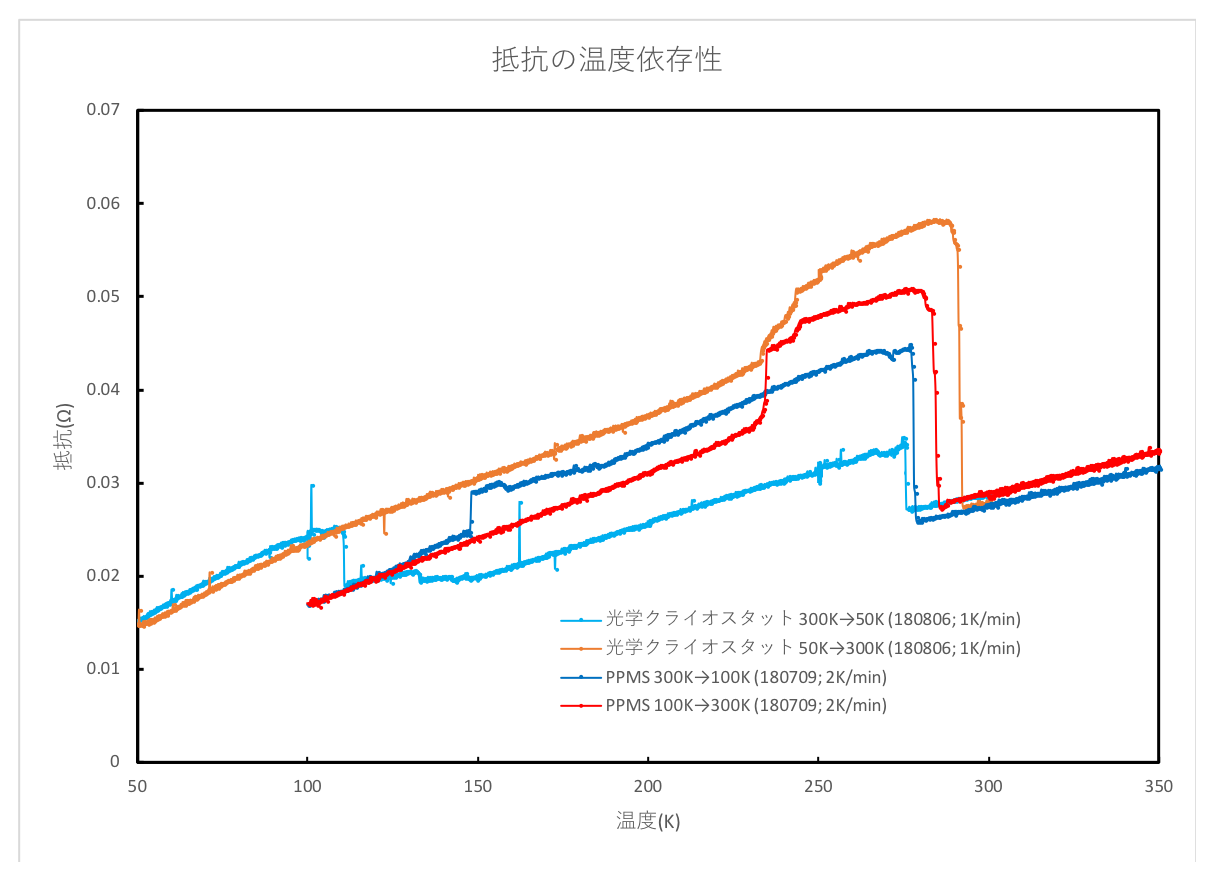
\includegraphics[width=150mm]{PPMS.eps}
  \end{center}
  \caption{PPMS実験と抵抗値の比較}
  \label{fig:PPMS}
\end{figure}
 
\subsection{偏光顕微光学系}
付録\ref{seq:BS_characterization}に示すように、本実験光学系で非偏光ビームスプリッタ(Thorlabs社製\#BSW41-532)を透過または反射する光には偏光に依存して位相差がつく。その偏光に依存した位相差に起因して、ビームスプリッタを透過または反射する光の偏光状態は変化する。例えば直線偏光をビームスプリッタに入射しても、透過する光は楕円偏光になってしまう。このような入射光の偏光状態の変化を避けるため、これまでビームスプリッタにp偏光(偏光が鉛直方向)かs偏光(偏光が水平方向)、無偏光のみを入射する条件で実験を行ってきた。しかし、結晶の対称性を明らかにするためには、入射光の偏光をより自由に制御する必要がある。図\ref{fig:microscope2}のように1/2波長板をビームスプリッタと対物レンズの間に置けば、ビームスプリッタにp偏光とs偏光のみを入射しながら、試料に入射する光の偏光をビームスプリッタより後方で制御することができる。この光学系を用いて入射光の偏光をより高い自由度で制御し、低温相の理解を深めることが今後の課題である。
\begin{figure}[htb]
  \begin{center}
   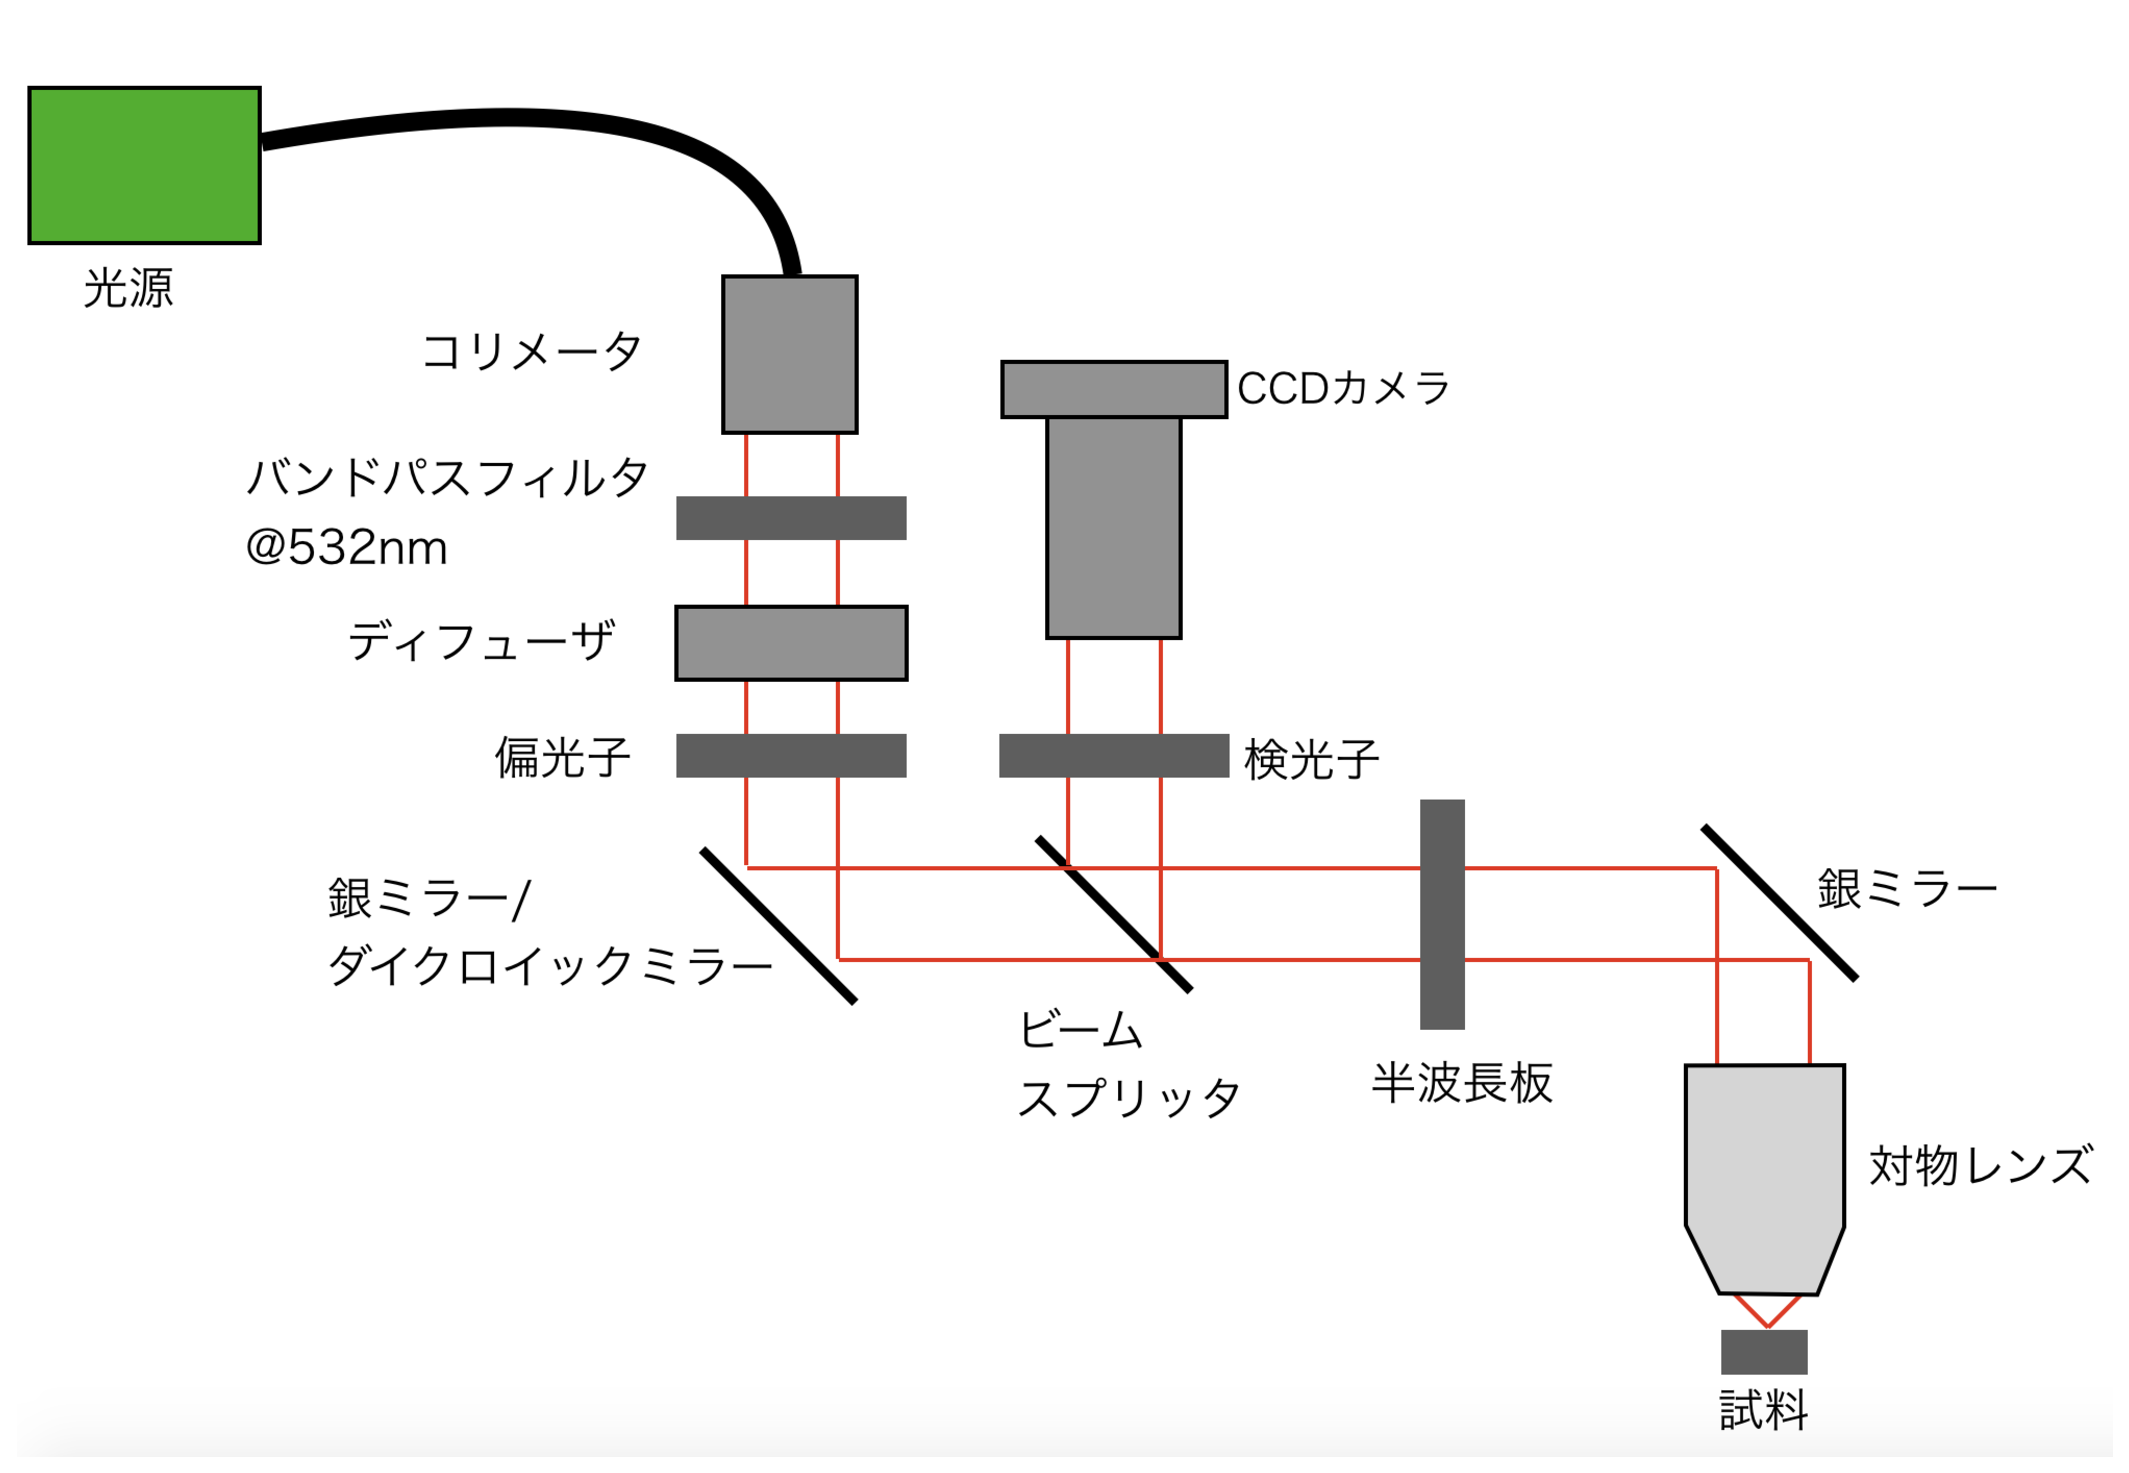
\includegraphics[width=120mm]{microscope2.eps}
  \end{center}
  \caption{改良された偏光顕微光学系の模式図}
  \label{fig:microscope2}
\end{figure}
